\documentclass[a4paper]{article}

\def\npart {III}
\def\nterm {Michaelmas}
\def\nyear {2017}
\def\nlecturer {M. Lis}
\def\ncourse {Advanced Probability}
\def\nnotready {}

% Imports
\ifx \nextra \undefined
  \usepackage[pdftex,
    hidelinks,
    pdfauthor={Dexter Chua},
    pdfsubject={Cambridge Maths Notes: Part \npart\ - \ncourse},
    pdftitle={Part \npart\ - \ncourse},
  pdfkeywords={Cambridge Mathematics Maths Math \npart\ \nterm\ \nyear\ \ncourse}]{hyperref}
  \title{Part \npart\ - \ncourse}
\else
  \usepackage[pdftex,
    hidelinks,
    pdfauthor={Dexter Chua},
    pdfsubject={Cambridge Maths Notes: Part \npart\ - \ncourse\ (\nextra)},
    pdftitle={Part \npart\ - \ncourse\ (\nextra)},
  pdfkeywords={Cambridge Mathematics Maths Math \npart\ \nterm\ \nyear\ \ncourse\ \nextra}]{hyperref}

  \title{Part \npart\ - \ncourse \\ {\Large \nextra}}
\fi

\author{Lectured by \nlecturer \\\small Notes taken by Dexter Chua}
\date{\nterm\ \nyear}

\usepackage{alltt}
\usepackage{amsfonts}
\usepackage{amsmath}
\usepackage{amssymb}
\usepackage{amsthm}
\usepackage{booktabs}
\usepackage{caption}
\usepackage{enumitem}
\usepackage{fancyhdr}
\usepackage{graphicx}
\usepackage{mathtools}
\usepackage{microtype}
\usepackage{multirow}
\usepackage{pdflscape}
\usepackage{pgfplots}
\usepackage{siunitx}
\usepackage{tabularx}
\usepackage{tikz}
\usepackage{tkz-euclide}
\usepackage[normalem]{ulem}
\usepackage[all]{xy}

\pgfplotsset{compat=1.12}

\pagestyle{fancyplain}
\lhead{\emph{\nouppercase{\leftmark}}}
\ifx \nextra \undefined
  \rhead{
    \ifnum\thepage=1
    \else
      \npart\ \ncourse
    \fi}
\else
  \rhead{
    \ifnum\thepage=1
    \else
      \npart\ \ncourse\ (\nextra)
    \fi}
\fi
\usetikzlibrary{arrows}
\usetikzlibrary{decorations.markings}
\usetikzlibrary{decorations.pathmorphing}
\usetikzlibrary{positioning}
\usetikzlibrary{fadings}
\usetikzlibrary{intersections}
\usetikzlibrary{cd}

\newcommand*{\Cdot}{\raisebox{-0.25ex}{\scalebox{1.5}{$\cdot$}}}
\newcommand {\pd}[2][ ]{
  \ifx #1 { }
    \frac{\partial}{\partial #2}
  \else
    \frac{\partial^{#1}}{\partial #2^{#1}}
  \fi
}

% Theorems
\theoremstyle{definition}
\newtheorem*{aim}{Aim}
\newtheorem*{axiom}{Axiom}
\newtheorem*{claim}{Claim}
\newtheorem*{cor}{Corollary}
\newtheorem*{defi}{Definition}
\newtheorem*{eg}{Example}
\newtheorem*{fact}{Fact}
\newtheorem*{law}{Law}
\newtheorem*{lemma}{Lemma}
\newtheorem*{notation}{Notation}
\newtheorem*{prop}{Proposition}
\newtheorem*{thm}{Theorem}

\renewcommand{\labelitemi}{--}
\renewcommand{\labelitemii}{$\circ$}
\renewcommand{\labelenumi}{(\roman{*})}

\let\stdsection\section
\renewcommand\section{\newpage\stdsection}

% Strike through
\def\st{\bgroup \ULdepth=-.55ex \ULset}

% Maths symbols
\newcommand{\bra}{\langle}
\newcommand{\ket}{\rangle}

\newcommand{\N}{\mathbb{N}}
\newcommand{\Z}{\mathbb{Z}}
\newcommand{\Q}{\mathbb{Q}}
\renewcommand{\H}{\mathbb{H}}
\newcommand{\R}{\mathbb{R}}
\newcommand{\C}{\mathbb{C}}
\newcommand{\Prob}{\mathbb{P}}
\renewcommand{\P}{\mathbb{P}}
\newcommand{\E}{\mathbb{E}}
\newcommand{\F}{\mathbb{F}}
\newcommand{\cU}{\mathcal{U}}
\newcommand{\RP}{\mathbb{RP}}
\newcommand{\CP}{\mathbb{CP}}

\newcommand{\ph}{\,\cdot\,}

\DeclareMathOperator{\sech}{sech}
\DeclareMathOperator{\cosech}{cosech}
\DeclareMathOperator{\cosec}{cosec}

\DeclareMathOperator{\covol}{covol}
\DeclareMathOperator{\vol}{vol}

\let\Im\relax
\let\Re\relax
\DeclareMathOperator{\Im}{Im}
\DeclareMathOperator{\Re}{Re}
\DeclareMathOperator{\im}{im}
\DeclareMathOperator{\image}{image}
\DeclareMathOperator{\Ann}{Ann}

\DeclareMathOperator*{\res}{res}
\DeclareMathOperator{\Res}{Res}
\DeclareMathOperator{\Ind}{Ind}

\DeclareMathOperator{\tr}{tr}
\DeclareMathOperator{\diag}{diag}
\DeclareMathOperator{\rank}{rank}
\DeclareMathOperator{\card}{card}
\DeclareMathOperator{\spn}{span}
\DeclareMathOperator{\adj}{adj}

\DeclareMathOperator{\erf}{erf}
\DeclareMathOperator{\erfc}{erfc}

\DeclareMathOperator{\ord}{ord}
\DeclareMathOperator{\Sym}{Sym}

\DeclareMathOperator{\sgn}{sgn}
\DeclareMathOperator{\orb}{orb}
\DeclareMathOperator{\stab}{stab}
\DeclareMathOperator{\ccl}{ccl}

\DeclareMathOperator{\lcm}{lcm}
\DeclareMathOperator{\hcf}{hcf}

\DeclareMathOperator{\Int}{Int}
\DeclareMathOperator{\id}{id}

\DeclareMathOperator{\betaD}{beta}
\DeclareMathOperator{\gammaD}{gamma}
\DeclareMathOperator{\Poisson}{Poisson}
\DeclareMathOperator{\binomial}{binomial}
\DeclareMathOperator{\multinomial}{multinomial}
\DeclareMathOperator{\Bernoulli}{Bernoulli}
\DeclareMathOperator{\like}{like}

\DeclareMathOperator{\var}{var}
\DeclareMathOperator{\cov}{cov}
\DeclareMathOperator{\bias}{bias}
\DeclareMathOperator{\mse}{mse}
\DeclareMathOperator{\corr}{corr}

\DeclareMathOperator{\otp}{otp}
\DeclareMathOperator{\dom}{dom}

\DeclareMathOperator{\Root}{Root}
\DeclareMathOperator{\supp}{supp}
\DeclareMathOperator{\rel}{rel}
\DeclareMathOperator{\Hom}{Hom}
\DeclareMathOperator{\Aut}{Aut}
\DeclareMathOperator{\Gal}{Gal}
\DeclareMathOperator{\Mat}{Mat}
\DeclareMathOperator{\End}{End}
\DeclareMathOperator{\Char}{char}
\DeclareMathOperator{\ev}{ev}
\DeclareMathOperator{\St}{St}
\DeclareMathOperator{\Lk}{Lk}
\DeclareMathOperator{\disc}{disc}
\DeclareMathOperator{\Isom}{Isom}
\DeclareMathOperator{\length}{length}
\DeclareMathOperator{\energy}{energy}
\DeclareMathOperator{\area}{area}
\DeclareMathOperator{\Syl}{Syl}
\DeclareMathOperator{\cl}{cl}
\DeclareMathOperator{\fix}{fix}

\newcommand{\GL}{\mathrm{GL}}
\newcommand{\SL}{\mathrm{SL}}
\newcommand{\PGL}{\mathrm{PGL}}
\newcommand{\PSL}{\mathrm{PSL}}
\newcommand{\PSU}{\mathrm{PSU}}
\newcommand{\Or}{\mathrm{O}}
\newcommand{\SO}{\mathrm{SO}}
\newcommand{\U}{\mathrm{U}}
\newcommand{\SU}{\mathrm{SU}}

\renewcommand{\d}{\mathrm{d}}
\newcommand{\D}{\mathrm{D}}

\tikzset{->/.style = {decoration={markings,
                                  mark=at position 1 with {\arrow[scale=2]{latex'}}},
                      postaction={decorate}}}
\tikzset{<-/.style = {decoration={markings,
                                  mark=at position 0 with {\arrowreversed[scale=2]{latex'}}},
                      postaction={decorate}}}
\tikzset{<->/.style = {decoration={markings,
                                   mark=at position 0 with {\arrowreversed[scale=2]{latex'}},
                                   mark=at position 1 with {\arrow[scale=2]{latex'}}},
                       postaction={decorate}}}
\tikzset{->-/.style = {decoration={markings,
                                   mark=at position #1 with {\arrow[scale=2]{latex'}}},
                       postaction={decorate}}}
\tikzset{-<-/.style = {decoration={markings,
                                   mark=at position #1 with {\arrowreversed[scale=2]{latex'}}},
                       postaction={decorate}}}

\tikzset{circ/.style = {fill, circle, inner sep = 0, minimum size = 3}}
\tikzset{mstate/.style={circle, draw, blue, text=black, minimum width=0.7cm}}

\definecolor{mblue}{rgb}{0.2, 0.3, 0.8}
\definecolor{morange}{rgb}{1, 0.5, 0}
\definecolor{mgreen}{rgb}{0.1, 0.4, 0.2}
\definecolor{mred}{rgb}{0.5, 0, 0}

\def\drawcirculararc(#1,#2)(#3,#4)(#5,#6){%
    \pgfmathsetmacro\cA{(#1*#1+#2*#2-#3*#3-#4*#4)/2}%
    \pgfmathsetmacro\cB{(#1*#1+#2*#2-#5*#5-#6*#6)/2}%
    \pgfmathsetmacro\cy{(\cB*(#1-#3)-\cA*(#1-#5))/%
                        ((#2-#6)*(#1-#3)-(#2-#4)*(#1-#5))}%
    \pgfmathsetmacro\cx{(\cA-\cy*(#2-#4))/(#1-#3)}%
    \pgfmathsetmacro\cr{sqrt((#1-\cx)*(#1-\cx)+(#2-\cy)*(#2-\cy))}%
    \pgfmathsetmacro\cA{atan2(#2-\cy,#1-\cx)}%
    \pgfmathsetmacro\cB{atan2(#6-\cy,#5-\cx)}%
    \pgfmathparse{\cB<\cA}%
    \ifnum\pgfmathresult=1
        \pgfmathsetmacro\cB{\cB+360}%
    \fi
    \draw (#1,#2) arc (\cA:\cB:\cr);%
}
\newcommand\getCoord[3]{\newdimen{#1}\newdimen{#2}\pgfextractx{#1}{\pgfpointanchor{#3}{center}}\pgfextracty{#2}{\pgfpointanchor{#3}{center}}}

\def\Xint#1{\mathchoice
   {\XXint\displaystyle\textstyle{#1}}%
   {\XXint\textstyle\scriptstyle{#1}}%
   {\XXint\scriptstyle\scriptscriptstyle{#1}}%
   {\XXint\scriptscriptstyle\scriptscriptstyle{#1}}%
   \!\int}
\def\XXint#1#2#3{{\setbox0=\hbox{$#1{#2#3}{\int}$}
     \vcenter{\hbox{$#2#3$}}\kern-.5\wd0}}
\def\ddashint{\Xint=}
\def\dashint{\Xint-}


\pgfdeclaredecoration{penciline}{initial}{
    \state{initial}[width=+\pgfdecoratedinputsegmentremainingdistance,auto corner on length=1mm,]{
        \pgfpathcurveto%
        {% From
            \pgfqpoint{\pgfdecoratedinputsegmentremainingdistance}
                            {\pgfdecorationsegmentamplitude}
        }
        {%  Control 1
        \pgfmathrand
        \pgfpointadd{\pgfqpoint{\pgfdecoratedinputsegmentremainingdistance}{0pt}}
                        {\pgfqpoint{-\pgfdecorationsegmentaspect\pgfdecoratedinputsegmentremainingdistance}%
                                        {\pgfmathresult\pgfdecorationsegmentamplitude}
                        }
        }
        {%TO
        \pgfpointadd{\pgfpointdecoratedinputsegmentlast}{\pgfpoint{1pt}{1pt}}
        }
    }
    \state{final}{}
}

\begin{document}
\maketitle
{\small
\setlength{\parindent}{0em}
\setlength{\parskip}{1em}

The aim of the course is to introduce students to advanced topics in modern probability theory. The emphasis is on tools required in the rigorous analysis of stochastic processes, such as Brownian motion, and in applications where probability theory plays an important role.

\noindent\textbf{Review of measure and integration:} sigma-algebras, measures and filtrations; integrals and expectation; convergence theorems; product measures, independence and Fubini's theorem.\\
\noindent\textbf{Conditional expectation:} Discrete case, Gaussian case, conditional density functions; existence and uniqueness; basic properties.\\
\noindent\textbf{Martingales:} Martingales and submartingales in discrete time; optional stopping; Doob's inequalities, upcrossings, martingale convergence theorems; applications of martingale techniques.\\
\noindent\textbf{Stochastic processes in continuous time:} Kolmogorov's criterion, regularization of paths; martingales in continuous time.\\
\noindent\textbf{Weak convergence:} Definitions and characterizations; convergence in distribution, tightness, Prokhorov's theorem; characteristic functions, L\'evy's continuity theorem.\\
\noindent\textbf{Sums of independent random variables:} Strong laws of large numbers; central limit theorem; Cram\'er's theory of large deviations.\\
\noindent\textbf{Brownian motion:} Wiener's existence theorem, scaling and symmetry properties; martingales associated with Brownian motion, the strong Markov property, hitting times; properties of sample paths, recurrence and transience; Brownian motion and the Dirichlet problem; Donsker's invariance principle.\\
\noindent\textbf{Poisson random measures:} Construction and properties; integrals.\\
\noindent\textbf{L\'evy processes:} L\'evy-Khinchin theorem.

\subsubsection*{Pre-requisites}
A basic familiarity with measure theory and the measure-theoretic formulation of probability theory is very helpful. These foundational topics will be reviewed at the beginning of the course, but students unfamiliar with them are expected to consult the literature (for instance, Williams' book) to strengthen their understanding.
}
\tableofcontents

\section{Introduction}
In some other places in the world, this course might be known as ``Stochastic Processes''. In addition to doing probability, a new component studied in the course is \emph{time}. We are going to study how things change over time.

In the first half of the course, we will focus on discrete time. We will have a discrete sequence of points, and we assign some random values to each of these points. The point, of course, is that there will be dependencies between the different points.

In the second half of the course, we will look at continuous time. There is a fundamental difference between the two, in that there is a nice topology on the interval. This allows us to say things like we want our trajectories to be continuous. However, we will see that to understand continuous time, we start with the corresponding discrete situation, and then try to ``take the limit'' as the sample points become closer and closer to each other. An important example is Brownian motion.

There are two main objects that appear in this course. The first is the conditional expectation. Recall that if we have a random variable $X$, we can obtain a number $\E[X]$, the expectation of $X$. We can think of this as integrating out all the randomness of the system. Conditional expectation will be some subtle modification of this construction, where we don't actually get a number, but another random variable. The idea behind this is that we want to integrate out some of the randomness in our random variable.

Another main object is \emph{stopping time}. For example, if we have a production line that produces random number of outputs at each point, then we can ask how much time it takes to produce a fixed number of goods, and this is a nice random time, which we call a stopping time. The niceness follows from the fact that if the time comes, we know it. An example that is not nice is, for example, the last day it rains in Cambridge in a particular month, since on that last day, we don't necessarily know that it is in fact the last day.

\section{Some measure theory}
\subsection{Review of measure theory}
To make the course as self-contained as possible, we shall begin with some review of measure theory. On the other hand, if one doesn't already know measure theory, they are recommended to learn the measure theory properly before starting this course.

\begin{defi}[$\sigma$-algebra]\index{$\sigma$-algebra}
  Let $E$ be a set. A subset $\mathcal{E}$ of the power set $\mathcal{P}(E)$ is called a \emph{$\sigma$-algebra} (or \term{$\sigma$-field}) if
  \begin{enumerate}
    \item $\emptyset \in \mathcal{E}$;
    \item If $A \in \mathcal{E}$, then $A^C = E \setminus A \in \mathcal{E}$;
    \item If $A_1, A_2, \ldots \in \mathcal{E}$, then $\bigcup_{n = 1}^\infty A_n \in \mathcal{E}$.
  \end{enumerate}
\end{defi}

\begin{defi}[Measurable space]\index{measurable space}
  A \emph{measurable space} is a set with a $\sigma$-algebra.
\end{defi}


\begin{defi}[Borel $\sigma$-algebra]\index{Borel $\sigma$-algebra}\index{$\sigma$-algebra!Borel}\index{$\mathcal{B}(E)$}
  Let $E$ be a topological space with topology $\mathcal{T}$. Then the \emph{Borel $\sigma$-algebra} $\mathcal{B}(E)$ on $E$ is the $\sigma$-algebra generated by $\mathcal{T}$, i.e.\ the smallest $\sigma$-algebra containing $\mathcal{T}$.
\end{defi}

We are often going to look at $\mathcal{B}(\R)$, and we will just write $\mathcal{B}$\index{$\mathcal{B}$} for it.

\begin{defi}[Measure]\index{measure}
  A function $\mu: \mathcal{E} \to [0, \infty]$ is a \emph{measure} if
  \begin{itemize}
    \item $\mu(\emptyset) = 0$
    \item If $A_1, A_2, \ldots \in \mathcal{E}$ are disjoint, then
      \[
        \mu \left(\bigcup_{i = 1}^\infty A_i \right) = \sum_{i = 1}^\infty \mu(A_i).
      \]
  \end{itemize}
\end{defi}

\begin{defi}[Measure space]\index{measure space}
  A \emph{measure space} is a measurable space with a measure.
\end{defi}

\begin{defi}[Measurable function]\index{measurable function}
  Let $(E_1, \mathcal{E}_1)$ and $(E_2, \mathcal{E}_2)$ be measurable spaces. Then $f: E_1 \to E_2$ is said to be \emph{measurable} if $A \in \mathcal{E}_2$ implies $f^{-1}(A) \in \mathcal{E}_1$.
\end{defi}
This is similar to the definition of a continuous function.

\begin{notation}\index{$m\mathcal{E}$}\index{$m\mathcal{E}^+$}
  For $(E, \mathcal{E})$ a measurable space, we write $m\mathcal{E}$ for the set of measurable functions $E \to \R$.

  We write $m\mathcal{E}^+$ to be the positive measurable functions, which are allowed to take value $\infty$.
\end{notation}
Note that we do \emph{not} allow taking the values $\pm \infty$ in the first case.

\begin{thm}
  Let $(E, \mathcal{E}, \mu)$ be a measure space. Then there exists a unique function $\tilde{\mu}: m\mathcal{E}^+ \to [0, \infty]$ satisfying
  \begin{itemize}
    \item $\tilde{\mu}(\mathbf{1}_A) = \mu(A)$, where $\mathbf{1}_A$ is the indicator function of $A$.
    \item Linearity: $\tilde{\mu}(\alpha f + \beta g) = \alpha \tilde{\mu}(f) + \beta \tilde{\mu}(g)$ if $\alpha, \beta \in \R_{\geq 0}$ and $f, g \in m\mathcal{E}^+$.
    \item Monotone convergence: iff $f_1, f_2, \ldots \in m\mathcal{E}^+$ are such that $f_n \nearrow f \in m\mathcal{E}^+$ pointwise a.e.\ as $n \to \infty$, then
      \[
        \lim_{n \to \infty} \tilde{\mu}(f_n) = \tilde{\mu} (f).
      \]
  \end{itemize}
  We call $\tilde{\mu}$ the \term{integral} with respect to $\mu$, and we will write it as $\mu$ from now on.
\end{thm}

\begin{defi}[Simple function]\index{simple function}
  A function $f$ is \emph{simple} if there exists $\alpha_n \in \R_{\geq 0}$ and $A_n \in \mathcal{E}$ for $1 \leq n \leq k$ such that
  \[
    f = \sum_{n = 1}^k \alpha_n \mathbf{1}_{A_n}.
  \]
\end{defi}
From the first two properties of the measure, we see that
\[
  \mu(f) = \sum_{n = 1}^k \alpha_n \mu(A_n).
\]
One convenient observation is that a function is simple iff it takes on only finitely many values. We then see that if $f \in m \mathcal{E}^+$, then
\[
  f_n = 2^{-n}\lfloor 2^n f\rfloor \wedge n
\]
is a sequence of simple functions approximating $f$ from below. Thus, given monotone convergence, this shows that
\[
  \mu(f) = \lim \mu(f_n),
\]
and this proves the uniqueness part of the theorem.

Recall that
\begin{defi}[Almost everywhere]\index{almost everywhere}
  We say $f = g$ almost everywhere if
  \[
    \mu(\{x \in E: f(x) \not= g(x)\}) = 0.
  \]
  We say $f$ is a \term{version} of $g$.
\end{defi}

\begin{eg}
  Let $\ell_n = \mathbf{1}_{[n, n + 1]}$. Then $\mu(\ell_n) = 1$ for all $1$, but also $f_n \to 0$ and $\mu(0) = 0$. So the ``monotone'' part of monotone convergence is important.
\end{eg}

So if the sequence is not monotone, then the measure does not preserve limits, but it turns out we still have an inequality.

\begin{lemma}[Fatou's lemma]\index{Fatou's lemma}
  Let $f_i \in m \mathcal{E}^+$. Then
  \[
    \mu\left(\liminf_n f_n\right) \leq \liminf_n \mu(f_n).
  \]
\end{lemma}

\begin{proof}
  Apply monotone convergence to the sequence $\inf_{m \geq n} f_m$
\end{proof}

Of course, it would be useful to extend integration to functions that are not necessarily positive.
\begin{defi}[Integrable function]\index{integrable function}
  We say a function $f \in m\mathcal{E}$ is \emph{integrable} if $\mu(|f|) \leq \infty$. We write \term{$L^1(E)$} (or just $L^1$) for the space of integrable functions.

  We extend $\mu$ to $L^1$ by
  \[
    \mu(f) = \mu(f^+) - \mu(f^-),
  \]
  where $f^{\pm} = (\pm f) \wedge 0$.
\end{defi}

If we want to be explicit about the measure and the $\sigma$-algebra, we can write $L^1(E, \mathcal{E} \mu)$.

\begin{thm}[Dominated convergence theorem]\index{dominated convergence theorem}
  If $f_i \in m\mathcal{E}$ and $f_i \to f$ a.e., such that there exists $g \in L^1$ such that $|f_i| \leq g$ a.e. Then
  \[
    \mu(f) = \lim \mu(f_n).
  \]
\end{thm}

\begin{proof}
  Apply Fatou's lemma to $g - f_n$ and $g + f_n$.
\end{proof}

\begin{defi}[Product $\sigma$-algebra]\index{product $\sigma$-algebra}\index{$\sigma$-algebra!product}
  Let $(E_1, \mathcal{E}_1)$ and $(E_2 , \mathcal{E}_2)$ be measure spaces. Then the product $\sigma$-algebra$ \mathcal{E}_1 \otimes \mathcal{E}_2$ is the smallest $\sigma$-algebra on $E_1 \times E_2$ containing all sets of the form $A_1 \times A_2$, where $A_i \in \mathcal{E}_i$.
\end{defi}

\begin{thm}
  If $(E_1, \mathcal{E}_1, \mu_1)$ and $(E_2, \mathcal{E}_2, \mu_2)$ are $\sigma$-finite measure spaces, then there exists a unique measure $\mu$ on $\mathcal{E}_1 \otimes \mathcal{E}_2)$ satisfying
  \[
    \mu(A_1 \times A_2) = \mu_1(A_1) \mu_2(A_2)
  \]
  for all $A_i \in \mathcal{E}_i$.

  This is called the \term{product measure}\index{measure!product}.
\end{thm}

\begin{thm}[Fubini's/Tonelli's theorem]\index{Fubini's theorem}\index{Tonelli's theorem}
  If $f = f(x_1, x_2) \in m\mathcal{E}^+$ with $\mathcal{E} = \mathcal{E}_1 \otimes \mathcal{E}_2$, then the functions
  \begin{align*}
    x_1 \mapsto \int f(x_1, x_2) \d \mu_2(x_2) \in m \mathcal{E}_1^+\\
    x_2 \mapsto \int f(x_1, x_2) \d \mu_1(x_1) \in m \mathcal{E}_2^+
  \end{align*}
  and
  \begin{align*}
    \int_E f \;\d u &= \int_{E_1} \left(\int_{E_2} f(x_1, x_2)\;\d \mu_2(x_2)\right) \d \mu_1(x_1)\\
    &= \int_{E_2} \left(\int_{E_1} f(x_1, x_2)\;\d \mu_1(x_1)\right) \d \mu_2(x_2)
  \end{align*}
\end{thm}
\subsection{Conditional expectation}
In this course, conditional expectation is going to play an important role, and it is worth spending some time developing the theory. We are going to focus on probability theory, which, mathematically, just means we assume $\mu(E) = 1$. Practically, it is common to change notation to $E = \Omega$, $\mathcal{E} = \mathcal{F}$, $\mu = \P$ and $\int\;\d \mu = \E$. Measurable functions will be written as $X, Y, Z$, and will be called \term{random variables}. Elements in $\mathcal{F}$ will be called \term{events}. An element $\omega \in \Omega$ will be called a \term{realization}.

There are many ways we can think about conditional expectations. The first one is how most of us first encountered conditional probability.

Suppose $B \in \mathcal{F}$, with $\P(B) > 0$. Then the conditional probability of the event $A$ given $B$ is
\[
  \P(A \mid B) = \frac{\P(A \cap B)}{\P(B)}.
\]
This should be interpreted as the probability that $A$ happened, given that $B$ happened. Since we assume $B$ happened, we ought to restrict to the subset of the probability space where $B$ in fact happened. To make this a probability space, we scale the probability measure by $\P(B)$. Then given any event $A$, we take the probability of $A \cap B$ under this probability measure, which is the formula given.

More generally, if $X$ is a random variable, the conditional expectation of $f$ given $B$ is just the expectation under this new probability measure,
\[
  \E[X \mid B] = \frac{\E[X \mathbf{1}_B]}{\P[B]}.
\]
We probably already know this from high school, and we are probably not quite excited by this. One natural generalization would be to allow $B$ to vary.

Let $G_1, G_2, \ldots \in \mathcal{F}$ be disjoint events such that $\bigcup_n G_n = \Omega$. Let
\[
  \mathcal{G} = \sigma(G_1, G_2, \ldots) = \left\{\bigcup_{n \in I} G_n: I \subseteq \N\right\}. % coarse graining
\]
Let $X \in L^1$. We then define
\[
  Y = \sum_{n = 1}^\infty \E(X \mid G_n) \mathbf{1}_{G_n}.
\]
Let's think about what this is saying. Suppose a random outcome $\omega$ happens. To compute $Y$, we figure out which of the $G_n$ our $\omega$ belongs to. Let's say $\omega \in G_k$. Then $Y$ returns the expected value of $X$ given that we live in $G_k$. In this processes, we have forgotten the exact value of $\omega$. All that matters is which $G_n$ the outcome belongs to. We can ``visually'' think of the $G_n$ as cutting up the sample space $\Omega$ into compartments:
\begin{center}
  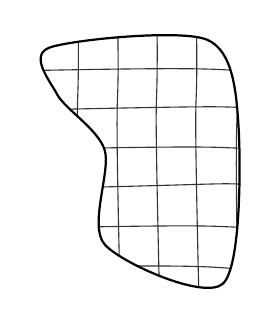
\begin{tikzpicture}
    \draw [thick] plot [smooth cycle] coordinates {(1.3, -1.2) (1.3, 0) (0.7, 0.7) (0.6, 1.3) (2.6, 1.4) (3, 0.3) (2.8, -1.7)};
    \clip plot [smooth cycle] coordinates {(1.3, -1.2) (1.3, 0) (0.7, 0.7) (0.6, 1.3) (2.6, 1.4) (3, 0.3) (2.8, -1.7)};
    \draw [step=0.5, opacity=0.8, decorate, decoration=penciline] (0, -2) grid (4, 1.7);
  \end{tikzpicture}
\end{center}
We then average out $X$ in each of these compartments to obtain $Y$. This is what we are going to call the conditional expectation of $X$ given $\mathcal{G}$, written $\E(X \mid \mathcal{G})$.

Ultimately, the characterizing property of $Y$ is the following lemma:
\begin{lemma}
  The conditional expectation $Y = \E(X \mid \mathcal{G})$ satisfies the following properties:
  \begin{itemize}
    \item $Y$ is $\mathcal{G}$-measurable
    \item We have $Y \in L^1$, and
      \[
        \E Y \mathbf{1}_A = \E X \mathbf{1}_A
      \]
      for all $A \in \mathcal{G}$.
  \end{itemize}
\end{lemma}

\begin{proof}
  It is clear that $Y$ is $\mathcal{G}$-measurable. To show it is $L^1$, we compute
  \begin{align*}
    \E[|Y|] &= \E \left|\sum_{n = 1}^\infty \E(X \mid G_n) \mathbf{1}_{G_n}\right|\\
    &\leq \E \sum_{n =1 }^\infty \E(|X| \mid G_n) \mathbf{1}_{G_n} \\
    &= \sum \E \left( \E(|X| \mid G_n) \mathbf{1}_{G_n}\right)\\
    &= \sum \E |X| \mathbf{1}_{G_n}\\
    &= \E \sum |X| \mathbf{1}_{G_n}\\
    &= \E |X|\\
    &< \infty,
  \end{align*}
  where we used monotone convergence twice to swap the expectation and the sum.

  The final part is also clear, since we can explicitly enumerate the elements in $\mathcal{G}$ and see that they all satisfy the last property.
\end{proof}

It turns out for any $\sigma$-subalgebra $\mathcal{G} \subseteq \mathcal{F}$, we can construct the conditional expectation $\E(X \mid \mathcal{G})$, which is uniquely characterized by the above two properties.

\begin{thm}[Existence and uniqueness of conditional expectation]
  Let $X \in L^1$, and $\mathcal{G} \subseteq \mathcal{F}$. Then there exists a random variable $Y$ such that
  \begin{itemize}
    \item $Y$ is $\mathcal{G}$-measurable
    \item $Y \in L^1$, and $\E X \mathbf{1}_A = \E Y \mathbf{1}_A$ for all $A \in \mathcal{G}$.
  \end{itemize}
  Moreover, if $Y'$ is another random variable satisfying these conditions, then $Y' = Y$ almost surely.

  We call $Y$ a (version of) the conditional expectation given $\mathcal{G}$.
\end{thm}

We will write the condition expectation as $\E(X \mid \mathcal{G})$, and if $X = \mathbf{1}_A$, we will write $\E(A \mid \mathcal{G}) = \E(\mathbf{1}_A \mid \mathcal{G})$.

Recall also that if $Z$ is a random variable, then $\sigma(Z) = \{Z^{-1}(B): B \in \mathcal{B}\}$. In this case, we will write $\E[X \mid Z) = \E(X \mid \sigma(Z))$.

By, say, bounded convergence, it follows from the second condition that $\E XZ = \E YZ$ for all bounded $\mathcal{G}$-measurable functions $Z$.
\begin{proof}
  We first consider the case where $X \in L^2(\Omega, \mathcal{F}, \mu)$. Then we know from functional analysis that for any $\mathcal{G} \subseteq \mathcal{F}$, the space $L^2(\mathcal{G})$ is a Hilbert space with inner product
  \[
    \langle X, Y \rangle = \mu (X Y).
  \]
  In particular, $L^2(\mathcal{G})$ is a closed subspace of $L^2(\mathcal{F})$. We can then define $Y$ to be the orthogonal projection of $X$ onto $L^2(\mathcal{G})$. It is immediate that $Y$ is $\mathcal{G}$-measurable. For the second part, we use that $X - Y$ is orthogonal to $L^2(\mathcal{G})$, since that's what orthogonal projection is supposed to be. So $\E(X - Y)Z = 0$ for all $Z \in L^2(\mathcal{G})$. In particular, since the measure space is finite, the indicator function of any measurable subset is $L^2$. So we are done.

  We next focus on the case where $X \in m\mathcal{E}^+$. We define
  \[
    X_n = X \wedge n
  \]
  We want to use monotone convergence to obtain our result. To do so, we need the following result:

  \begin{claim}
    If $(X, Y)$ and $(X', Y')$ satisfy the conditions of the theorem, and $X' \geq X$ a.s., then $Y' \geq Y$ a.s.
  \end{claim}

  \begin{proof}
    Define the event $A = \{Y' \leq Y\} \in \mathcal{G}$. Consider the event $Z = (Y - Y')\mathbf{1}_A$. Then $Z \geq 0$. We then have
    \[
      \E Y' \mathbf{1}_A = \E X' \mathbf{1}_A \geq \E X \mathbf{1}_A = \E Y \mathbf{1}_A.
    \]
    So it follows that we also have $\E(Y - Y')\mathbf{1}_A \leq 0$. So in fact $\E Z = 0$. So $Y' \geq Y$ a.s.
  \end{proof}
  We can now define $Y_n = \E(X_n \mid \mathcal{G})$, picking them so that $\{Y_n\}$ is increasing. We then take $Y_\infty = \lim Y_n$. Then $Y_\infty$ is certainly $\mathcal{G}$-measurable, and by monotone convergence, if $A \in \mathcal{G}$, then
  \[
    \E X \mathbf{1}_A = \lim \E X_n \mathbf{1}_A = \lim \E Y_n \mathbf{1}_A = \E Y_\infty \mathbf{1}_A.
  \]
  Now if $\E X < \infty$, then $\E Y_\infty = \E X < \infty$. So we know $Y_\infty$ is finite a.s., and we can define $Y = Y_\infty \mathbf{1}_{Y_\infty < \infty}$.

  Finally, we work with arbitrary $X \in L^1$. We can write $X = X^+ - X^-$, and then define $Y^\pm = \E (X^\pm \mid \mathcal{G})$, and take $Y = Y^+ - Y^-$.

  Uniqueness is then clear.
\end{proof}

\begin{lemma}
  If $Y$ is $\sigma(Z)$-measurable, then there exists $h: \R \to \R$ Borel-measurable such that $Y = h(Z)$. In particular,
  \[
    \E(X \mid Z) = h(Z) \text{ a.s.}
  \]
  for some $h: \R \to \R$.
\end{lemma}
We can then define $\E(X \mid Z = z) = h(z)$. The point of doing this is that we want to allow for the case where in fact we have $\P(Z = z) = 0$, in which case our original definition does not make sense.

\begin{ex}
  Consider $X \in L^1$, and $Z: \Omega \to \N$ discrete. Compute $\E(X \mid Z)$ and compare our different definitions of conditional expectation.
\end{ex}

\begin{eg}
  Let $(U, V) \in \R^2$ with density $f_{U, V}(u, v)$, so that for any $B_1, B_2 \in \mathcal{B}$, we have
  \[
    \P(U \in B_1, V \in B_2) = \int_{B_1} \int_{b_2} f_{U, V}(u, v) \;\d u \;\d v.
  \]
  We want to compute $\E(h(V) \mid U)$, where $h: \R \to \R$ is Borel measurable. We can define
  \[
    f_U(u) = \int_\R f_{U, V} (u, v) \;\d v,
  \]
  and we define the conditional density of $V$ given $U$ by
  \[
    F_{ \mid U} (v \mid u) = \frac{f_{U, V}(u, v)}{f_U(u)}.
  \]
  We define
  \[
    g(u) = \int h(u) f_{V \mid U} (v \mid u)\;\d v.
  \]
  We claim that $\E(h(V) \mid U)$ is just $g(U)$.

  To check this, we show that it satisfies the two desired conditions. It is clear that it is $\sigma(U)$-measurable. To check the second condition, fix an $A \in \sigma(U)$. Then $A = \{(u, v): u \in B\}$ for some $B$. Then
  \begin{align*}
    \E(h(V) \mathbf{1}_A) &= \iint h(v) \mathbf{1}_{u \in B} f_{U, V} (u, v)\;\d u\;\d v\\
    &= \iint h(v) \mathbf{1}_{u \in B} f_{V \mid U}(v \mid u) f_V(u)\;\d u\;\d v\\
    &= \int g(U) \mathbf{1}_{u \in B} f_U(u) \;\d u\\
    &= \E(g(U) \mathbf{1}_A),
  \end{align*}
  as desired.
\end{eg}
The point of this example is that to compute conditional expectations, we use our intuition to guess what the conditional expectation should be, and then check that it satisfies the two uniquely characterizing properties.

\begin{eg}
  Suppose $(X, W)$ are Gaussian. Then for all linear functions $\varphi: \R^2 \to \R$, the quantity $\varphi(X, W)$ is Gaussian.

  One nice property of Gaussians is that lack of correlation implies independence. We want to compute $\E(X \mid W)$. Note that if $Y$ is such that $\E X = \E Y$, $X - Y$ is independent of $W$, and $Y$ is $W$-measurable, then $Y = \E(X \mid W)$, since
  $\E(X - Y) \mathbf{1}_A = 0$ for all $\sigma(W)$-measurable $A$.

  The guess is that we want $Y$ to be a Gaussian variable. We put $Y = aW + b$. Then $\E X = \E Y$ implies we must have
  \[
    a \E W + b = \E X.\tag{$*$}
  \]
  The independence part requires $\cov(X - Y, W) = 0$. Since covariance is linear, we have
  \[
    0 = \cov(X - Y, W) = \cov(X, W) - \cov(aW + b, W) = \cov(X, W) - a \cov(W, W).
  \]
  Recalling that $\cov(W, W) = \var(W)$, we need
  \[
    a = \frac{\cov(X, W)}{\var(W)}.
  \]
  This then allows us to use $(*)$ to compute $b$ as well. This is how we compute the conditional expectation of Gaussians.
\end{eg}

We note some immediate properties of conditional expectation. As usual, all (in)equality and convergence statements are to be taken with the quantifier ``almost surely''.
\begin{prop}\leavevmode
  \begin{enumerate}
    \item $\E(X \mid \mathcal{G}) = X$ iff $X$ is $\mathcal{G}$-measurable.
    \item $\E(\E(X \mid \mathcal{G})) = \E X$
    \item If $X \geq 0$ a.s., then $\E(X \mid \mathcal{G}) \geq 0$
    \item If $X$ and $\mathcal{G}$ are independent, then $\E(X \mid \mathcal{G}) = \E[X]$
    \item If $\alpha, \beta \in \R$ and $X_1, X_2 \in L^1$, then
      \[
        \E(\alpha X_1 + \beta X_2 \mid \mathcal{G}) = \alpha \E(X_1 \mid\mathcal{G}) + \beta \E(X_2 \mid \mathcal{G}).
      \]
    \item Suppose $X_n \nearrow X$. Then
      \[
        \E(X_n\mid \mathcal{G}) \nearrow \E(X \mid \mathcal{G}).
      \]
    \item \term{Fatou's lemma}: If $X_n$ are non-negative measurable, then
      \[
        \E\left(\liminf_{n \to \infty} X_n \mid \mathcal{G}\right) \leq \liminf_{n \to \infty} \E(X_n \mid \mathcal{G}).
      \]
    \item \emph{Dominated convergence theorem}\index{dominated convergence theorem}: If $X_n \to X$ and $Y \in L^1$ such that $Y \geq |X_n|$ for all $n$, then
      \[
        \E(X_n \mid \mathcal{G}) \to \E(X \mid \mathcal{G}).
      \]
    \item \term{Jensen's inequality}: If $c: \R \to \R$ is convex, then
      \[
        \E(c(X) \mid \mathcal{G}) \geq c(\E(X) \mid \mathcal{G}).
      \]
    \item \emph{Tower property}\index{tower property}: If $\mathcal{H} \subseteq \mathcal{G}$, then
      \[
        \E(\E(X \mid \mathcal{G}) \mid \mathcal{H}) = \E(X \mid \mathcal{H}).
      \]
    \item For $p \geq 1$,
      \[
        \|\E(X \mid \mathcal{G})\|_p \leq \|X\|_p.
      \]
    \item If $Z$ is bounded and $\mathcal{G}$-measurable, then
      \[
        \E(ZX \mid \mathcal{G}) = Z \E(X \mid \mathcal{G}).
      \]
    \item Let $X \in L^1$ and $\mathcal{G}, \mathcal{H} \subseteq \mathcal{F}$. Assume that $\sigma(X, \mathcal{G})$ is independent of $\mathcal{H}$. Then
      \[
        \E (X \mid \mathcal{G}) = \E(X \mid \sigma(\mathcal{G}, \mathcal{H})).
      \]
  \end{enumerate}
\end{prop}

\begin{proof}\leavevmode
  \begin{enumerate} % actually check these
    \item Clear.
    \item Take $A = \omega$.
    \item Shown in the proof.
    \item Clear by property of expected value of independent variables.
    \item Clear, since the RHS satisfies the unique characterizing property of the LHS.
    \item Clear from construction.
    \item Same as the unconditional proof, using the previous property.
    \item Same as the unconditional proof, using the previous property.
    \item Same as the unconditional proof.
    \item The LHS satisfies the characterizing property of the RHS
    \item Using the convexity of $|x|^p$, Jensen's inequality tells us
      \begin{align*}
        \|E(X \mid \mathcal{G})\|_p^p &= \E |\E(X \mid \mathcal{G})|^p\\
        &\leq \E (\E (|X|^p \mid \mathcal{G}))\\
        &= \E |X|^p\\
        &= \|X\|_p^p
      \end{align*}
    \item If $Z = \mathbf{1}_B$, and let $b \in \mathcal{G}$. Then
      \[
        \E(Z \E(X \mid \mathcal{G}) \mathbf{1}_A) = \E (\E (X \mid \mathcal{G}) \cdot \mathbf{1}_{A \cap B}) = \E(X \mathbf{1}_{A \cap B}) = \E(Z X \mathbf{1}_A).
      \]
      So the lemma holds. Linearity then implies the result for $Z$ simple, then apply our favorite convergence theorems.
    \item Take $B \in \mathcal{H}$ and $A \in \mathcal{G}$. Then
      \begin{align*}
        \E(\E(X \mid \sigma(\mathcal{G}, \mathcal{H}))\cdot \mathbf{1}_{A \cap B}) &= \E(X \cdot \mathbf{1}_{A \cap B})\\
        &= \E(X \mathbf{1}_A) \P(B)\\
        &= \E(\E(X \mid \mathcal{G}) \mathbf{1}_A) \P(B)\\
        &= \E(\E(X \mid \mathcal{G}) \mathbf{1}_{A \cap B})
      \end{align*}
      If instead of $A \cap B$, we had any $\sigma(\mathcal{G}, \mathcal{H})$-measurable set, then we would be done. But we are fine, since the set of subsets of the form $A \cap B$ with $A \in \mathcal{G}$, $B \in \mathcal{H}$ is a generating $\pi$-system for $\sigma(\mathcal{H}, \mathcal{G})$. \qedhere
  \end{enumerate}
\end{proof}

We shall end with the following key lemma. We will later use it to show that many of our \emph{martingales} are uniformly integrable.
\begin{lemma}
  If $X \in L^1$, then the family of random variables $Y_{\mathcal{G}} = \E(X \mid \mathcal{G})$ for all $\mathcal{G} \subseteq \mathcal{F}$ is uniformly integrable.

  In other words, for all $\varepsilon > 0$, there exists $\lambda > 0$ such that
  \[
    \E(Y_{\mathcal{G}} \mathbf{1}_{|Y_{\mathcal{G}} > \lambda|}) < \varepsilon
  \]
  for all $\mathcal{G}$.
\end{lemma}

\begin{proof}
  Fix $\varepsilon > 0$. Then there exists $\delta > 0$ such that $\E |X|\mathbf{1}_A < \varepsilon$ for any $A$ with $\P(A) < \delta$.

  Take $Y = \E (X \mid \mathcal{G})$. Then by Jensen, we know
  \[
    |Y| \leq \E(|X| \mid \mathcal{G})
  \]
  In particular, we have
  \[
    \E|Y| \leq \E|X|.
  \]
  By Markov's inequality, we have
  \[
    \P(|Y| \geq \lambda) \leq \frac{\E|Y|}{\lambda} \leq \frac{\E|X|}{\lambda}.
  \]
  So take $\lambda$ such that $\frac{\E|X|}{\lambda} < \delta$. So we have
  \[
    \E(|Y| \mathbf{1}_{|Y| \geq \lambda}) \leq \E(\E(|X| \mid \mathcal{G})\mathbf{1}_{|Y| \geq \lambda}) = \E(|X| \mathbf{1}_{|Y| \geq \lambda}) < \varepsilon
  \]
  using that $\mathbf{1}_{|Y| \geq \lambda}$ is a $\mathcal{G}$-measurable function.
\end{proof}

\section{Martingales in discrete time}
\subsection{Filtrations and martingales}
We would like to model some random variable that ``evolves with time''. For example, in a simple random walk, $X_n$ could be the position we are at time $n$. To do so, we would like to have some $\sigma$-algebras $\mathcal{F}_n$ that tells us the ``information we have at time $n$''. This structure is known as a \emph{filtration}.

\begin{defi}[Filtration]\index{filtration}
  A \emph{filtration} is a sequence of $\sigma$-algebras $(\mathcal{F}_n)_{n \geq 0}$ such that $\mathcal{F} \supseteq \mathcal{F}_{n + 1} \supseteq \mathcal{F}_n$ for all $n$. We define $\mathcal{F}_\infty = \sigma(\mathcal{F}_0, \mathcal{F}_1, \ldots) \subseteq \mathcal{F}$.
\end{defi}

We will from now on assume $(\Omega, \mathcal{F}, \P)$ is equipped with a filtration $(\mathcal{F}_n)_{n \geq 0}$.

\begin{defi}[Stochastic process in discrete time]\index{discrete stochastic process}\index{stochastic process!discrete}
  A \emph{stochastic process} (in discrete time) is a sequence of random variables $(X_n)_{n \geq 0}$.
\end{defi}

This is a very general definition, and in most cases, we would want $X_n$ to interact nicely with our filtration.
\begin{defi}[Natural filtration]\index{natural filtration}\index{filtration!natural}
  The \emph{natural filtration} of $(X_n)_{n \geq 0}$ is given by
  \[
    \mathcal{F}_n^X = \sigma(X_1, \ldots, X_n).
  \]
\end{defi}

\begin{defi}[Adapted process]\index{adapted process}\index{stochastic process!adapted}
  We say that $(X_n)_{n \geq 0}$ is \emph{adapted} (to $(\mathcal{F}_n)_{n \geq 0}$) if $X_n$ is $\mathcal{F}_n$-measurable for all $n \geq 0$. Equivalently, if $\mathcal{F}^X_n \subseteq \mathcal{F}_n$.
\end{defi}

\begin{defi}[Integrable process]\index{integrable process}\index{stochastic process!integrable}
  A process $(X_n)_{n \geq 0}$ is \emph{integrable} if $X_n \in L^1$ for all $n \geq 0$.
\end{defi}

We can now write down the definition of a martingale.
\begin{defi}[Martingale]\index{martingale}
  An integrable adapted process $(X_n)_{n \geq 0}$ is a \emph{martingale} if for all $n \geq m$, we have
  \[
    \E(X_n \mid \mathcal{F}_m) = X_m.
  \]
  We say it is a \term{super-martingale} if
  \[
    \E(X_n \mid \mathcal{F}_m) \leq X_m,
  \]
  and a \term{sub-martingale} if
  \[
    \E(X_n \mid \mathcal{F}_m) \geq X_m,
  \]
\end{defi}
Note that it is enough to take $m = n - 1$ for all $n \geq 0$, using the tower property.

The idea of a martingale is that we cannot predict whether $X_n$ will go up or go down in the future even if we have all the information up to the present. For example, if $X_n$ denotes the wealth of a gambler in a gambling game, then in some sense $(X_n)_{n \geq 0}$ being a martingale means the game is ``fair'' (in the sense of a fair dice).

Note that $(X_n)_{n \geq 0}$ is a super-martingale iff $(-X_n)_{n \geq 0}$ is a sub-martingale, and if $(X_n)_{n \geq 0}$ is a martingale, then it is both a super-martingale and a sub-martingale. Often, what these extra notions buy us is that we can formulate our results for super-martingales (or sub-martingales), and then by applying the result to both $(X_n)_{n \geq 0}$ and $(-X_n)_{n \geq 0}$, we obtain the desired, stronger result for martingales.

\subsection{Stopping time and optimal stopping}
The optional stopping theorem says the definition of a martingale in fact implies an \emph{a priori} much stronger property. To formulate the optional stopping theorem, we need the notion of a stopping time.

\begin{defi}[Stopping time]\index{stopping time}
  A \emph{stopping time} is a random variable $T: \Omega \to \N_{ \geq 0} \cup \{\infty\}$ such that
  \[
    \{T \leq n\} \in \mathcal{F}_n
  \]
  for all $n \geq 0$.
\end{defi}
This means that at time $n$, if we want to know if $T$ has occurred, we can determine it using the information we have at time $n$.

Note that $T$ is a stopping time iff $\{t = n \} \in \mathcal{F}_n$ for all $n$, since if $T$ is a stopping time, then
\[
  \{T = n\} = \{T \leq n\} \setminus \{T \leq n - 1\},
\]
and $\{T \leq n- 1\} \in \mathcal{F}_{n - 1} \subseteq \mathcal{F}_n$. Conversely,
\[
  \{T \leq n \} = \bigcup_{k = 1}^n \{T = k\} \in \mathcal{F}_n.
\]
This will not be true in the continuous case.

\begin{eg}
  If $B \in \mathcal{B}(\R)$, then we can define
  \[
    T = \inf \{n : X_n \in B\}.
  \]
  Then this is a stopping time.

  On the other hand,
  \[
    T = \sup \{n: X_n \in B\}
  \]
  is not a stopping time (in general).
\end{eg}

Given a stopping time, we can make the following definition:
\begin{defi}[$X_T$]\index{$X_T$}
  For a stopping time $T$, we define the random variable $X_T$ by
  \[
    X_T (\omega) = X_{T(\omega)}(\omega)
  \]
  on $\{T < \infty\}$, and $0$ otherwise.
\end{defi}
Later, for suitable martingales, we will see that the limit $X_\infty = \lim_{n \to \infty} X_n$ makes sense. In that case, We define $X_T(\omega)$ to be $X_\infty(\omega)$ if $T = \infty$.

Similarly, we can define
\begin{defi}[Stopped process]\index{stopped process}
  The \emph{stopped process} is defined by
  \[
    (X_n^T)_{n \geq 0} = (X_{T(\omega) \wedge n}(\omega))_{n \geq 0}.
  \]
\end{defi}
This says we stop evolving the random variable $X$ once $T$ has occurred.

We would like to say that $X_T$ is ``$\mathcal{F}_T$-measurable'', i.e.\ to compute $X_T$, we only need to know the information up to time $T$. After some thought, we see that the following is the correct definition of $\mathcal{F}_T$:
\begin{defi}[$\mathcal{F}_T$]\index{$\mathcal{F}_T$}
  For a stopping time $T$, define
  \[
    \mathcal{F}_T = \{A \in \mathcal{F}_\infty : A \cap \{T \leq n\} \in \mathcal{F}_n\}.
  \]
\end{defi}
This is easily seen to be a $\sigma$-algebra.

\begin{eg}
  If $T \equiv n$ is constant, then $F\mathcal{F}_T = \mathcal{F}_n$.
\end{eg}

There are some fairly immediate properties of these objects, whose proof is left as an exercise for the reader:
\begin{prop}\leavevmode
  \begin{enumerate}
    \item If $T, S, (T_n)_{n \geq 0}$ are all stopping times, then
      \[
        T \vee S, T \wedge S, \sup_n T_n, \inf T_n, \limsup T_n, \liminf T_n
      \]
      are all stopping times.
    \item $\mathcal{F}_T$ is a $\sigma$-algebra
    \item If $S \leq T$, then $\mathcal{F}_S \subseteq \mathcal{F}_T$.
    \item $X_T \mathbf{1}_{T < \infty}$ is $\mathcal{F}_T$-measurable.
    \item If $(X_n)$ is an adapted process, then so is $(X^T_n)_{n \geq 0}$ for any stopping time $T$.
    \item If $(X_n)$ is an integrable process, then so is $(X^T_n)_{n \geq 0}$ for any stopping time $T$.\qedsym
  \end{enumerate}
\end{prop}

We now come to the fundamental property of martingales.
\begin{thm}[Optional stopping theorem]\index{optional stopping theorem}
  Let $(X_n)_{n \geq 0}$ be a super-martingale and $S \leq T$ \emph{bounded} stopping times. Then
  \[
    \E X_T \leq \E X_S.
  \]
\end{thm}

\begin{proof}
  Follows from the next theorem.
\end{proof}
What does this theorem mean? If $X$ is a martingale, then it is both a super-martingale and a sub-martingale. So we can apply this to both $X$ and $-X$, and so we have
\[
  \E(X_T) = \E(X_S).
\]
In particular, since $0$ is a stopping time, we see that
\[
  \E X_T = \E X_0
\]
for \emph{any} bounded stopping time $T$.

Recall that martingales are supposed to model fair games. If we again think of $X_n$ as the wealth at time $n$, and $T$ as the time we stop gambling, then this says no matter how we choose $T$, as long as it is bounded, the expected wealth at the end is the same as what we started with.

\begin{eg}
  Consider the stopping time
  \[
    T = \inf \{n : X_n = 1\},
  \]
  and take $X$ such that $\E X_0 = 0$. Then clearly we have $\E X_T = 1$. So this tells us $T$ is not a bounded stopping time!
\end{eg}

\begin{thm}
  The following are equivalent:
  \begin{enumerate}
    \item $(X_n)_{n \geq 0}$ is a super-martingale.
    \item For any bounded stopping times $T$ and any stopping time $S$,
      \[
        \E(X_T \mid \mathcal{F}_S) \leq X_{S \wedge T}.
      \]
    \item $(X_n^T)$ is a super-martingale for any stopping time $T$.
    \item For bounded stopping times $S, T$ such that $S \leq T$, we have
      \[
        \E X_T \leq \E X_S.
      \]
  \end{enumerate}
\end{thm}
In particular, (iv) implies (i).

\begin{proof}\leavevmode
  \begin{itemize}
    \item (ii) $\Rightarrow$ (iii): Consider $(X_n^{T'})_{ \geq 0}$ for a stopping time $T'$. To check if this is a super-martingale, we need to prove that whenever $m \leq n$,
      \[
        \E(X_{n \wedge T'} \mid \mathcal{F}_m) \leq X_{m \wedge T'}.
      \]
      But this follows from (ii) above by taking $S = m$ and $T = T' \wedge n$.
    \item (ii) $\Rightarrow$ (iv): Clear by the tower law.
    \item (iii) $\Rightarrow$ (i): Take $T = \infty$.
    \item (i) $\Rightarrow$ (ii): Assume $T \leq n$. Then
      \begin{align*}
        X_T &= X_{S \wedge T} + \sum_{S \leq k < T} (X_{k + 1} - X_k)\\
        &= X_{S \wedge T} + \sum_{k = 0}^n (X_{k + 1} - X_k) \mathbf{1}_{S \leq k < T} \tag{$*$}
      \end{align*}
      Now note that $\{S \leq k < T\} = \{S \leq k\} \cap \{T \leq k\}^c \in \mathcal{F}_k$. Let $A \in \mathcal{F}_S$. Then $A \cap \{S \leq k\} \in \mathcal{F}_k$ by definition of $\mathcal{F}_S$. So $A \cap \{S \leq k < T\} \in \mathcal{F}_k$.

      Apply $\E$ to to $(*) \times \mathbf{1}_A$. Then we have
      \[
        \E (X_T \mathbf{1}_A) = \E(X_{S \wedge T} \mathbf{1}_A) + \sum_{k = 0}^n \E(X_{k + 1} - X_k) \mathbf{1}_{A \cap \{S \leq k < T\}}.
      \]
      But for all $k$, we know
      \[
        \E(X_{k + 1} - X_k) \mathbf{1}_{A \cap \{S \leq k < T\}} \leq 0,
      \]
      since $X$ is a super-martingale. So it follows that for all $A \in \mathcal{F}_S$, we have
      \[
        \E(X_T \cdot \mathbf{1}_A) \leq \E(X_{S \wedge T} \mathbf{1}_A).
      \]
      But since $X_{S \wedge T}$ is $\mathcal{F}_{S \wedge T}$ measurable, it is in particular $\mathcal{F}_S$ measurable. So it follows that for all $A \in \mathcal{F}_S$, we have
      \[
        \E(\E (X_T \mid \mathcal{F}_S) \mathbf{1}_A) \leq \E(X_{S \wedge T} \mathbf{1}_A).
      \]
      So the result follows.
    \item (iv) $\Rightarrow$ (i): Fix $m \leq n$ and $A \in \mathcal{F}_m$. Take
      \[
        T = m \mathbf{1}_A + \mathbf{1}_{A^C}.
      \]
      One then manually checks that this is a stopping time. Now note that
      \[
        X_T = X_m \mathbf{1}_{A} + X_n \mathbf{1}_{A^C}.
      \]
      So we have
      \begin{align*}
        0 &\geq \E(X_n) - \E(X_T) \\
        &= \E(X_n) - \E(X_n \mathbf{1}_{A^c}) - \E(X_m \mathbf{1}_A) \\
        &= \E (X_n \mathbf{1}_A) - \E (X_m \mathbf{1}_A).
      \end{align*}
      Then the same argument as before gives the result.\qedhere
  \end{itemize}
\end{proof}

\subsection{Martingale convergence theorems}
One particularly nice property of martingales is that they have nice convergence properties. We shall begin by proving a pointwise version of martingale convergence.

\begin{thm}[Almost sure martingale convergence theorem]\index{martingale convergence theorem!almost sure}
  Suppose $(X_n)_{n \geq 0}$ is a super-martingale that is bounded in $L^1$, i.e.\ $\sup_n \E|X_n| < \infty$. Then there exists an $\mathcal{F}_\infty$-measurable $X_\infty \in L^1$ such that
  \[
    X_n \to X_\infty\text{ a.s. as }n \to \infty.
  \]
\end{thm}

To begin, we need a convenient characterization of when a series converges.
\begin{defi}[Upcrossing]\index{upcrossing}
  Let $(x_n)$ be a sequence and $(a, b)$ an interval. An \emph{upcrossing} of $(a, b)$ by $(x_n)$ is a sequence $j, j + 1, \ldots, k$ such that $x_j \leq a$ and $x_k \geq b$. We define\index{$U_n[a, b, (x_n)]$}\index{$U[a, b, (x_n)$}
  \begin{align*}
    U_n[a, b, (x_n)] &= \text{number of disjoint upcrossings contained in }\{1, \ldots, n\}\\
    U[a, b, (x_n)] &= \lim_{n \to \infty} U_n[a, b, x].
  \end{align*}
\end{defi}

We can then make the following elementary observation:
\begin{lemma}
  Let $(x_n)_{n \geq 0}$ be a sequence of numbers. Then $x_n$ converges in $\R$ if and only if
  \begin{enumerate}
    \item $\liminf |x_n| < \infty$.
    \item For all $a, b \in \Q$ with $a < b$, we have $U[a, b, (x_n)] < \infty$.
  \end{enumerate}
\end{lemma}
For our martingales, since they are bounded in $L^1$, Fatou's lemma tells us $\E \liminf |X_n| < \infty$. So $\liminf |X_n| = 0$ almost surely. Thus, it remains to show that for any fixed $a < b \in \Q$, we have $\P(U[a, b, (X_n)] = \infty) = 0$. This is a consequence of Doob's upcrossing lemma.

\begin{lemma}[Doob's upcrossing lemma]\index{Doob's upcrossing lemma}
  If $X_n$ is a super-martingale, then
  \[
    (b - a) \E(U_n[a, b(X_n)]) \leq \E(X_n - a)^-
  \]
\end{lemma}

\begin{proof}
  Assume that $X$ is a positive super-martingale. We define stopping times $S_k, T_k$ as follows:
  \begin{itemize}
    \item $T_0 = 0$
    \item $S_{k + 1} = \inf\{n: X_n \leq a, n \geq T_n\}$
    \item $T_{k + 1} = \inf\{n: X_n \geq b, n \geq S_{k + 1}\}$.
  \end{itemize}
  Given an $n$, we want to count the number of upcrossings before $n$. There are two cases we might want to distinguish:
  \begin{center}
    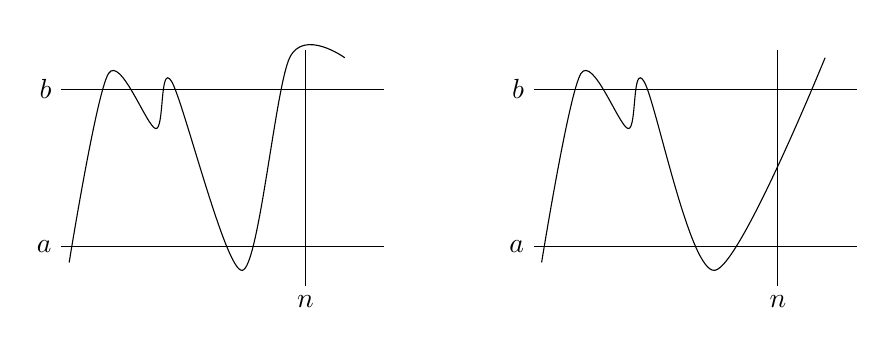
\begin{tikzpicture}
      \draw (-0.1, 0) node [left] {$b$} -- (4, 0);
      \draw (-0.1, -2) node [left] {$a$} -- (4, -2);
      \draw (3, -2.5) node [below] {$n$} -- (3, 0.5);

      \draw plot [smooth] coordinates {(0, -2.2) (0.5, 0.2) (1.1, -0.5) (1.3, 0.1) (2.2, -2.3) (2.8, 0.4) (3.5, 0.4)};

      \begin{scope}[shift={(6, 0)}]
        \draw (-0.1, 0) node [left] {$b$} -- (4, 0);
        \draw (-0.1, -2) node [left] {$a$} -- (4, -2);
        \draw (3, -2.5) node [below] {$n$} -- (3, 0.5);

        \draw plot [smooth] coordinates {(0, -2.2) (0.5, 0.2) (1.1, -0.5) (1.3, 0.1) (2.2, -2.3) (3.6, 0.4)};
      \end{scope}
    \end{tikzpicture}
  \end{center}
  Now consider the sum
  \[
    \sum_{k = 1}^n X_{T_k \wedge n} - X_{S_k \wedge n}.
  \]
  In the first case, this is equal to
  \[
    \sum_{k = 1}^{U_n} X_{T_k} - X_{S_k} + \sum_{k = U_n + 1}^n X_n - X_n \geq (b - a) U_n.
  \]
  In the second case, it is equal to
  \[
    \sum_{k = 1}^{U_n} X_{T_k} - X_{S_k} + (X_n - X_{S_{U_n + 1}}) + \sum_{k = U_n + 2}^n X_n - X_n \geq (b - a) U_n + (X_n - X_{S_{U_n + 1}}).
  \]
  Thus, in general, we have
  \[
    \sum_{k = 1}^n X_{T_k \wedge n} - X_{S_k \wedge n} \geq (b - a) U_n + (X_n - X_{S_{U_n + 1} \wedge n}).
  \]
  By definition, $S_k < T_k \leq n$. So the expectation of the LHS is always non-negative by super-martingale convergence, and thus
  \[
    0 \geq (b - a) \E U_n + \E(X_n - X_{S_{U_n + 1} \wedge n}).
  \]
  Then observe that
  \[
    X_n- X_{S_{U_n + 1}} \geq - (X_n - a)^-.
  \]
\end{proof}
%
%\begin{proof}[Proof of theorem]
%  Define
%  \[
%    \Omega_\infty = \{\omega: \limsup (X_n(\omega))< \infty\}.
%  \]
%  Moreover, for all $a < b \in \R$, define
%  \[
%    \Omega_{a, b} = \{\omega: U[a, b, (X_n)] < \infty\}.
%  \]
%  By our lemma, we know that $X_n$ converges on
%  \[
%    \Omega_\infty \cap \left(\cap_{a < b \in \Q} \Omega_{a, b}\right).
%  \]
%  Moreover, by Doob's upcrossings lemma, we know
%  \[
%    \P\left(\Omega_\infty \cap \left(\cap_{a < b \in \Q} \Omega_{a, b}\right)\right) = 1
%  \]
%  since we are taking a countable intersection.
%\end{proof}

The almost-sure martingale convergence theorem is very nice, but often it is not good enough. For example, we might want convergence in $L^p$ instead. The following example shows this isn't always possible:

\begin{eg}
  Suppose $(\rho_n)_{n \geq 0}$ is a sequence of iid random variables and
  \[
    \P(\rho_n = 0) = \frac{1}{2} = \P(\rho_n = 2).
  \]
  Let
  \[
    X_n = \prod_{k = 0}^n \rho_k.
  \]
  Then this is a martingale, and $\E X_n = 1$. On the other hand, $X_n \to 0$ almost surely. So $\|X_n - X_\infty\|_1$ does not converge to $0$.
\end{eg}

For $p > 1$, if we want convergence in $L^p$, it is not surprising that we at least need the sequence to be $L^p$ bounded. We will see that this is in fact sufficient. For $p = 1$, however, we need a bit more than being bounded in $L^1$. We will need uniform integrability.

To prove this, we need to establish some inequalities.
\begin{lemma}[Maximal inequality]\index{maximal inequality}
  Let $(X_n)$ be a sub-martingale that is non-negative, or a martingale. Define
  \[
    X^*_n = \sup_{k \leq n} |X_k|,\quad X^* = \lim_{n \to \infty} X_n^*.
  \]
  If $\lambda \geq 0$, then
  \[
    \lambda \P(X_n^* \geq \lambda) \leq \E[|X_n|\mathbf{1}_{X_n^* \geq \lambda}].
  \]
  In particular, we have
  \[
    \lambda \P(X_n^* \geq \lambda) \leq \E[|X_n|].
  \]
\end{lemma}
Markov's inequality says almost the same thing, but has $\E[|X_n^*|]$ instead of $\E[|X_n|]$. So this is a stronger inequality.

\begin{proof}
  If $X_n$ is a martingale, then $|X_n|$ is a sub-martingale. So it suffices to consider the case of a non-negative sub-martingale. We define the stopping time
  \[
    T = \inf\{n: X_n \geq \lambda\}.
  \]
  By optional stopping,
  \begin{align*}
    \E X_n &\geq \E X_{T \wedge n} \\\qedhere
    &= \E X_T \mathbf{1}_{T \leq n} + \E X_n \mathbf{1}_{T > n}\\
    &\geq \lambda \P(T \leq n) + \E X_n \mathbf{1}_{T > n}\\
    &= \lambda \P(X_n^* \geq \lambda) + \E X_n \mathbf{1}_{T > n}.\qedhere
  \end{align*}
\end{proof}

\begin{lemma}[Doob's $L^p$ inequality]\index{Doob's $L^p$ inequality}\index{$L^p$ inequality}
  For $p > 1$, we have
  \[
    \|X_n^*\|_p \leq \frac{p}{p - 1} \|X_n\|_p
  \]
  for all $n$.
\end{lemma}

\begin{proof}
  Let $k > 0$, and consider
  \[
    \|X_n^* \wedge k \|^p_p = \E |X_n^* \wedge k|^p.
  \]
  We use the fact that
  \[
    x^p = \int_0^x p s^{p - 1}\;\d s.
  \]
  So we have
  \begin{align*}
    \|X_n^* \wedge k\|^p_p &= \E|X_n^* \wedge k|^p\\
    &= \E \int_0^{X_n^* \wedge k} p x^{p - 1}\;\d x\\
    &= \E \int_0^k p x^{p - 1} \mathbf{1}_{X_n^* \geq x}\;\d x\\
    &= \int_0^k p x^{p - 1} \P(X_n^* \geq x)\;\d x\tag{Fubini}\\
    &\leq \int_0^k px^{p - 2} \E X_n \mathbf{1}_{X_n^* \geq x} \;\d x\tag{maximal inequality}\\
    &= \E X_n \int_0^k p x^{p - 2} \mathbf{1}_{X_n^* \geq x}\;\d x \tag{Fubini}\\
    &= \frac{p}{p - 1} \E X_n (X_n^* \wedge k) ^{p - 1}\\
    &\leq \frac{p}{p - 1} \|X_n\|_p \left(\E(X_n^* \wedge k)^p\right)^{\frac{p - 1}{p}}\tag{H\:older}\\
    &= \frac{p}{p - 1} \|X_n\|_p \|X_n^* \wedge k\|_p^{p - 1}
  \end{align*}
  Now take the limit $k \to \infty$ and divide by $\|X_n^*\|_p^{p - 1}$.
\end{proof}

\begin{thm}[$L^p$ martingale convergence theorem]\index{martingale convergence theorem!$L^p$}
  Let $(X_n)_{n \geq 0}$ be a martingale, and $p > 1$. Then the following are equivalent:
  \begin{enumerate}
    \item $(X_n)_{n \geq 0}$ is bounded in $L^p$, i.e.\ $\sup_n \E |X_i|^p < \infty$.
    \item $(X_n)_{n \geq 0}$ converges as $n \to \infty$ to a random variable $X_\infty \in L^p$ almost surely and in $L^p$.
    \item There exists a random variable $Z \in L^p$ such that
      \[
        X_n = \E (Z \mid \mathcal{F}_n)
      \]
  \end{enumerate}
  Moreover, in (iii), we always have $X_\infty = \E(Z \mid \mathcal{F}_\infty)$.
\end{thm}
This gives a bijection between martingales bounded in $L^p$ and $L^p(\mathcal{F}_\infty)$, sending $(X_n)_{n \geq 0} \mapsto X_\infty$.

\begin{proof}\leavevmode
  \begin{itemize}
    \item (i) $\Rightarrow$ (ii): If $(X_n)_{n \geq 0}$ is bounded in $L^p$, then it is bounded in $L^1$. So by the martingale convergence theorem, we know $(X_n)_{n \geq 0}$ converges almost surely to $X_\infty$. By Fatou's lemma, we have $X_\infty \in L^p$.

      Now by monotone convergence, we have
      \[
        \|X^*\|_p = \lim_n \|X_n^*\|_p \leq \frac{p}{p - 1} \sup_n \|X_n\|_p < \infty.
      \]
      By the triangle inequality, we have
      \[
        |X_n - X_\infty| \leq 2 X^*\text{ a.s.}
      \]
      So by dominated convergence, we know that $X_n \to X_\infty$ in $L^p$.
    \item (ii) $\Rightarrow$ (iii): Take $Z = X_\infty$. We want to prove that
      \[
        X_m = \E(X_\infty \mid \mathcal{F}_m).
      \]
      To do so, we show that $\|X_m - \E(X_\infty \mid \mathcal{F}_m)\|_p = 0$. For $n \geq m$, we know this is equal to
      \[
        \|E(X_n \mid \mathcal{F}_m) - \E(X_\infty \mid \mathcal{F}_m)\|_p = \|\E(X_n - X_\infty \mid \mathcal{F}_m)\|_p \leq \|X_n - X_\infty\|_p \to 0
      \]
      as $n \to \infty$, where the last step uses Jensen's. But it is also a constant. So we are done.
    \item (iii) $\Rightarrow$ (i): Since expectation decreases $L^p$ norms, we already know that $(X_n)_{n \geq 0}$ is $L^p$-bounded.

      To show the ``moreover'' part, note that $\bigcup_{n \geq 0} \mathcal{F}_n$ is a $\pi$-system that generates $\mathcal{F}_\infty$. So it is enough to prove that
      \[
        \E X_\infty \mathbf{1}_A = \E(\E(Z \mid \mathcal{F}_\infty) \mathbf{1}_A).
      \]
      But if $A \in \mathcal{F}_N$, then
      \begin{align*}
        \E X_\infty \mathbf{1}_A &= \lim_{n \to \infty} \E X_n \mathbf{1}_A\\
        &= \lim_{n \to \infty} \E(\E(Z \mid \mathcal{F}_n) \mathbf{1}_A)\\
        &= \lim_{n \to \infty} \E (\E(Z \mid \mathcal{F}_\infty)\mathbf{1}_A),
      \end{align*}
      where the last step relies on the fact that $\mathbf{1}_A$ is $\mathcal{F}_n$-measurable.
  \end{itemize}
\end{proof}

We finally finish off the $p = 1$ case with the additional uniform integrability condition.
\begin{thm}[Convergence in $L^1$]\index{martingale convergence theorem!$L^1$}
  Let $(X_n)_{n \geq 0}$ be a martingale. Then the following are equivalent:
  \begin{enumerate}
    \item $(X_n)_{n \geq 0}$ is uniformly integrable.
    \item $(X_n)_{n \geq 0}$ converges almost surely and in $L^1$.
    \item There exists $Z \in L^1$ such that $X_n = \E(Z \mid \mathcal{F}_n)$ almost surely.
  \end{enumerate}
  Moreover, $X_\infty = \E(Z \mid F_\infty)$.
\end{thm}

The proof is very similar to the $L^p$ case.
\begin{proof}\leavevmode
  \begin{itemize}
    \item (i) $\Rightarrow$ (ii): Let $(X_n)_{n \geq 0}$ be uniformly integrable. Then $(X_n)_{n \geq 0}$ is bounded in $L^1$. So the $(X_n)_{n \geq 0}$ converges to $X_\infty$ almost surely. Then by measure theory, uniform integrability implies that in fact $X_n \to L^1$.
    \item (ii) $\Rightarrow$ (iii): Same as the $L^p$ case.
    \item (iii) $\Rightarrow$ (i): For any $Z \in L^1$, the collection $\E(Z \mid \mathcal{G})$ ranging over all $\sigma$-subalgebras $\mathcal{G}$ is uniformly integrable.
  \end{itemize}
\end{proof}
Thus, there is a bijection between uniformly integrable martingales and $L^1(\mathcal{F}_\infty)$.

We now revisit optional stopping for uniformly integrable martingales. Recall that in the statement of optional stopping, we needed our stopping times to be bounded. It turns out if we require our martingales to be uniformly integrable, then we can drop this requirement.

\begin{thm}
  If $(X_n)_{n \geq 0}$ is a uniformly integrable martingale, and $S, T$ are arbitrary stopping times, then $\E(X_T \mid \mathcal{F}_S) = X_{S \wedge T}$. In particular $\E X_T = X_0$.
\end{thm}
Note that we are now allowing arbitrary stopping times, so $T$ may be infinite with non-zero probability. Hence we define
\[
  X_T = \sum_{n = 0}^\infty X_n \mathbf{1}_{T = n} + X_\infty \mathbf{1}_{T = \infty}.
\]

\begin{proof}
  By optional stopping, for every $n$, we know that
  \[
    \E (X_{T \wedge n} \mid \mathcal{F}_S) = X_{S \wedge T \wedge n}.
  \]
  We want to be able to take the limit as $n \to \infty$. To do so, we need to show that things are uniformly integrable. First, we apply optional stopping to write $X_{T \wedge n}$ as
  \begin{align*}
    X_{T\wedge n} &= \E(X_n \mid \mathcal{F}_{T \wedge n})\\
    &= \E(\E(X_\infty \mid \mathcal{F}_n) \mid \mathcal{F}_{T \wedge n})\\
    &= \E(X_\infty \mid \mathcal{F}_{T \wedge n}).
  \end{align*}
  So we know $(X_n^T)_{n \geq 0}$ is uniformly integrable, and hence $X_{n \wedge T} \to X_T$ almost surely and in $L^1$.

  To understand $\E (X_{T \wedge n} \mid \mathcal{F}_S)$, we note that
  \[
    \|\E(X_{n \wedge T} - X_T \mid \mathcal{F}_S)\|_1 \leq \|X_{n \wedge T} - X_T \|_1 \to 0\text{ as }n \to \infty.
  \]
  So it follows that $\E(X_{n \wedge T} \mid \mathcal{F}_S) \to \E(X_T \mid \mathcal{F}_S)$ as $n \to \infty$.
\end{proof}

\subsection{Applications of martingales}
Having developed the theory, let us move on to some applications. Before we do that, we need the notion of a \emph{backwards martingale}.
\begin{defi}[Backwards filtration]\index{backwards filtration}\index{filtration!backwards}
  A \emph{backwards filtration} on a measurable space $(E, \mathcal{E})$ is a sequence of $\sigma$-algebras $\hat{\mathcal{F}}_n \subseteq \mathcal{E}$ such that $\hat{F}_{n + 1} \subseteq \hat{F}_n$. We define
  \[
    \hat{\mathcal{F}}_\infty = \bigcap_{n \geq 0} \hat{\mathcal{F}}_n.
  \]
\end{defi}

\begin{thm}
  Let $Y \in L^1$, and let $\hat{\mathcal{F}}_n$ be a backwards filtration. Then
  \[
    \E(Y \mid \hat{\mathcal{F}}_n) \to \E(Y \mid \hat{\mathcal{F}}_\infty)
  \]
  almost surely and in $L^1$.
\end{thm}
A process of this form is known as a \term{backwards martingale}.

\begin{proof}
  We first show that $\E(Y \mid \hat{F}_n)$ converges. We then show that what it converges to is indeed $\E(Y \mid \hat{\mathcal{F}}_\infty)$.

  We write
  \[
    X_n = \E(Y \mid \hat{\mathcal{F}}_n).
  \]
  Observe that for all $n \geq 0$, the process $(X_{n - k})_{0 \leq k \leq n}$ is a martingale by the tower property, and so is $(-X_{n - k})_{0 \leq k \leq n}$. Now notice that for all $a < b$, the number of upcrossings of $[a, b]$ by $(X_k)_{0 \leq k \leq n}$ is equal to the number of upcrossings of $[-b, -a]$ by $(-X_{n - k})_{0 \leq k \leq n}$.

  Using the same arguments as for martingales, we conclude that $X_n \to X_\infty$ almost surely and in $L^1$ for some $X_\infty$.

  To see that $X_\infty = \E(Y \mid \hat{\mathcal{F}}_\infty)$, we notice that $X_\infty$ is $\hat{F}_\infty$ measurable. So it is enough to prove that
  \[
    \E X_\infty \mathbf{1}_A = \E(\E(Y \mid \hat{\mathcal{F}}_\infty) \mathbf{1}_A)
  \]
  for all $A \in \hat{\mathcal{F}}_\infty$. Indeed, we have
  \begin{align*}
    \E X_\infty \mathbf{1}_A &= \lim_{n \to \infty} \E X_n \mathbf{1}_A\\
    &= \lim_{n\to \infty} \E(\E (Y \mid \hat{\mathcal{F}}_n) \mathbf{1}_A)\\
    &= \lim_{n \to \infty} \E(Y \mid \mathbf{1}_A)\\
    &= \E(Y \mid \mathbf{1}_A)\\
    &= \E(\E (Y \mid \hat{\mathcal{F}}_n) \mathbf{1}_A).\qedhere
  \end{align*}
\end{proof}


\begin{thm}[Kolmogorov 0-1 law]\index{Kolmogorov 0-1 law}
  Let $(X_n)_{n \geq 0}$ be independent random variables. Then, let
  \[
    \hat{\mathcal{F}}_n = \sigma (X_{n + 1}, X_{n + 2}, \ldots).
  \]
  Then the \term{tail $\sigma$-algebra} $\hat{\mathcal{F}}_{\infty}$ is trivial\index{trivial $\sigma$-algebra}\index{$\sigma$-algebra!trivial}, i.e.\ $\P(A) \in \{0, 1\}$ for all $A \in \hat{\mathcal{F}}_\infty$.
\end{thm}

\begin{proof}
  Let $\mathcal{F}_n = \sigma(X_1, \ldots, X_n)$. Then $\mathcal{F}_n$ and $\hat{\mathcal{F}}_n$ are independent. Then for all $A \in \hat{\mathcal{F}}_\infty$, we have
  \[
    \E(\mathbf{1}_A \mid \mathcal{F}_n) = \P(A).
  \]
  But the LHS is a martingale. So it converges almost surely and in $L^1$ to $\E(\mathbf{1}_A \mid \mathcal{F}_\infty)$. But $\mathbf{1}_A$ is $\mathcal{F}_\infty$-measurable, since $\hat{\mathcal{F}}_\infty \subseteq \mathcal{F}_\infty$. So this is just $\mathbf{1}_A$. So $\mathbf{1}_A = \P(A)$ almost surely, and we are done.
\end{proof}

\begin{thm}[Strong law of large numbers]
  Let $(X_n)_{n \geq 1}$ be iid random variables in $L^1$, with $\E X_1 = \mu$. Define
  \[
    S_n = \sum_{i = 1}^n X_i.
  \]
  Then
  \[
    \frac{S_n}{n} \to \mu\text{ as }n \to \infty
  \]
  almost surely and in $L^1$.
\end{thm}

\begin{proof}
  We have
  \[
    S_n = \E(S_n \mid S_n) = \sum_{i = 1}^n \E(X_i \mid S_n) = n \E(X_1 \mid S_n).
  \]
  So the problem is equivalent to showing that $\E(X_1 \mid S_n) \to \mu$ as $n \to \infty$. This seems like something we can tackle with our existing technology, except that the $S_n$ do not form a filtration.

  Thus, define a backwards filtration
  \[
    \hat{\mathcal{F}}_n = \sigma(S_n, S_{n + 1}, S_{n + 2}, \ldots) = \sigma(S_n, X_{n + 1}, X_{n + 2}, \ldots) = \sigma(S_n, \tau_n),
  \]
  where $\tau_n = \sigma(X_{n + 1}, X_{n + 2}, \ldots)$. We now use the property of conditional expectation that we've never used so far, that adding independent information to a conditional expectation doesn't change the result. Since $\tau_n$ is independent of $\sigma(X_1, S_n)$, we know
  \[
    \frac{S_n}{n} = \E(X_1 \mid S_n) = \E(X_1 \mid \hat{\mathcal{F}}_n).
  \]
  Thus, by backwards martingale convergence, we know
  \[
    \frac{S_n}{n} \to \E(X_1 \mid \hat{\mathcal{F}}_{\infty}).
  \]
  But by the Kolmogorov 0-1 law, we know $\hat{\mathcal{F}}_{\infty}$ is trivial. So we know that $\E(X_1 \mid \hat{\mathcal{F}}_{\infty})$ is almost constant, which has to be $\E(\E(X_1 \mid \hat{\mathcal{F}}_{\infty})) = \E(X_1) = \mu$.
\end{proof}

Recall that if $(E, \mathcal{E}, \mu)$ is a measure space and $f \in m\mathcal{E}^+$, then
\[
  \nu(A) = \mu(f \mathbf{1}_A)
\]
is a measure on $\mathcal{E}$. We say $f$ is a density of $\nu$ with respect to $\mu$.

We can ask an ``inverse'' question -- given two different measures on $\mathcal{E}$, when is it the case that one is given by a density with respect to the other?

A first observation is that if $\nu(A) = \mu(f \mathbf{1}_A)$, then whenever $\mu(A) = 0$, we must have $\nu(A) = 0$. However, this is not sufficient. For example, let $\mu$ be a counting measure on $\R$, and $\nu$ the Lebesgue measure. Then our condition is satisfied. However, if $\nu$ is given by a density $f$ with respect to $\nu$, we must have
\[
  0 = \nu(\{x\}) = \mu(f \mathbf{1}_{\{x\}}) = f(x).
\]
So $f \equiv 0$, but taking $f \equiv 0$ clearly doesn't give the Lebesgue measure.

The problem with this is that $\mu$ is not a $\sigma$-finite measure.

\begin{thm}[Radon--Nikodym]\index{Radon--Nikodym theorem}
  Let $(\Omega, \mathcal{F})$ be a measurable space, and $\Q$ and $\P$ be two probability measures on $(\Omega, \mathcal{F})$. Then the following are equivalent:
  \begin{itemize}
    \item $\Q$ is absolutely continuous with respect to $\P$, i.e.\ for any $A \in \mathcal{F}$, if $\P(A) = 0$, then $\Q(A) = 0$.
    \item For any $\varepsilon > 0$, there exists $\delta > 0$ such that for all $A \in \mathcal{F}$, if $\P(A) \leq \delta$, then $\Q(A) \leq \varepsilon$.
    \item There exists a random variable $X \geq 0$ such that
      \[
        \Q(A) = \E_{\P}(X \mathbf{1}_A).
      \]
      In this case, $X$ is called the \term{Radon--Nikodym derivative} of $\Q$ with respect to $\P$, and we write $X = \frac{\d \Q}{\d \P}$.
  \end{itemize}
\end{thm}
Note that this theorem works for all finite measures by scaling, and thus for $\sigma$-finite measures by partitioning $\Omega$ into sets of finite measure.

\begin{proof}
  We shall only treat the case where $\mathcal{F}$ is \emph{countably generated}\index{countably generated $\sigma$-algebra}\index{$\sigma$-algebra!countably generated}, i.e.\ $\mathcal{F} = \sigma(F_1, F_2, \ldots)$ for some sets $F_i$. For example, any second-countable topological space is countably generated.
  \begin{itemize}
    \item (iii) $\Rightarrow$ (i): Clear.
    \item (ii) $\Rightarrow$ (iii): Define the filtration
      \[
        \mathcal{F}_n = \sigma(F_1, F_2, \ldots, F_n).
      \]
      Since $\mathcal{F}_n$ is finite, we can write it as
      \[
        \mathcal{F}_n = \sigma(A_{n, 1}, \ldots, A_{n, m_n}),
      \]
      where each $A_{n, i}$ is an \term{atom}, i.e.\ if $B \subsetneq A_{n, i}$ and $B \in \mathcal{F}_n$, then $B = \emptyset$. We define
      \[
        X_n = \sum_{n = 1}^{m_n} \frac{\Q(A_{n, i})}{\P(A_{n, i})} \mathbf{1}_{A_{n, i}},
      \]
      where we skip over the terms where $\P(A_{n, i}) = 0$. Note that this is exactly designed so that for any $A \in \mathcal{F}_n$, we have
      \[
        \E_\P (X_n \mathbf{1}_A) = \E_\P \sum_{A_{n, i} \subseteq A} \frac{\Q(A_{n, i})}{\P(A_n, i)} \mathbf{1}_{A_{n, i}} = \Q(A).
      \]
      Thus, if $A \in \mathcal{F}_n \subseteq \mathcal{F}_{n + 1}$, we have
      \[
        \E X_{n + 1} \mathbf{1}_A = \Q(A) = \E X_n \mathbf{1}_A.
      \]
      So we know that
      \[
        \E(X_{n + 1} \mid \mathcal{F}_n) = X_n.
      \]
      It is also immediate that $(X_n)_{n \geq 0}$ is adapted. So it is a martingale.

      We next show that $(X_n)_{n \geq 0}$ is uniformly integrable. By Markov's inequality, we have
      \[
        \P(X_n \geq \lambda) \leq \frac{\E X_n}{\lambda} = \frac{1}{\lambda}\leq \delta
      \]
      for $\lambda$ large enough. Then
      \[
        \E(X_n \mathbf{1}_{X_n \geq \lambda}) = \Q(X_n \geq \lambda) \leq \varepsilon.
      \]
      So we have shown uniform integrability, and so we know $X_n \to X$ almost surely and in $L^1$ for some $X$. Then for all $A \in \bigcup_{n \geq 0} \mathcal{F}_n$, we have
      \[
        \Q(A) = \lim_{n \to \infty} \E X_n \mathbf{1}_A = \E X \mathbf{1}_A.
      \]
      So $\Q(-)$ and $\E X \mathbf{1}_{(-)}$ agree on $\bigcup_{n \geq 0} \mathcal{F}_n$, which is a generating $\pi$-system for $\mathcal{F}$, so they must be the same.
    \item (i) $\Rightarrow$ (ii): Suppose not. Then there exists some $\varepsilon > 0$ and some $A_1, A_2, \ldots \in \mathcal{F}$ such that
      \[
        \Q(A_n) \geq \varepsilon,\quad \P(A_n) \leq \frac{1}{2^n}.
      \]
      Since $\sum_n \P(A_n)$ is finite, by Borel--Cantelli, we know
      \[
        \P \limsup A_n = 0.
      \]
      On the other hand, by, say, dominated convergence, we have
      \begin{align*}
        \Q\limsup A_n &= \Q \left(\bigcap_{n = 1}^\infty \bigcup_{m = n}^\infty A_m\right) \\
        &= \lim_{k \to \infty} \Q\left(\bigcap_{n = 1}^k \bigcup_{m = n}^\infty A_m \right)\\
        &\geq \lim_{k \to \infty} \Q \left(\bigcup_{m = k}^\infty A_k\right)\\
        &\geq \varepsilon.
      \end{align*}
      This is a contradiction.\qedhere
  \end{itemize}
\end{proof}

Finally, we end the part on discrete time processes by relating what we have done to Markov chains.

Let's first recall what Markov chains are. Let $E$ be a countable space, and $\mu$ a measure on $E$. We write $\mu_x = \mu(\{x\})$, and then $\mu(f) = \mu \cdot f$.

\begin{defi}[Transition matrix]\index{transition matrix}
  A \emph{transition matrix} is a matrix $P = (p_{xy})_{x, y \in E}$ such that each $p_x = (p_{x, y})_{y \in E}$ is a probability measure on $E$.
\end{defi}

\begin{defi}[Markov chain]\index{Markov chain}
  An adapted process $(X_n)$ is called a \emph{Markov chain} if for any $n$ and $A \in \mathcal{F}_n$ such that $\{x_n = x\} \supseteq A$, we have
  \[
    \P(X_{n + 1} = y\mid A) = p_{xy}.
  \]
\end{defi}

\begin{defi}[Harmonic function]\index{harmonic function}
  A function $f: E \to \R$ is \emph{harmonic} if $Pf = f$. In other words, for any $x$, we have
  \[
    \sum_{y} p_{xy} f(y) = f(x).
  \]
\end{defi}
We then observe that

\begin{prop}
  if $F$ is harmonic and bounded, and $(X_n)_{n \geq 0}$ is Markov, then $(f(x_n))_{n \geq 0}$ is a martingale.
\end{prop}

\begin{eg}
  Let $(X_n)_{n \geq 0}$ be iid $\Z$-valued random variables in $L^1$, and $\E[X_i] = 0$. Then
  \[
    S_n = X_0 + \cdots + X_n
  \]
  is a martingale and a Markov chain.

  However, if $Z$ is a $\Z$-valued random variable, consider the random variable $(ZS_n)_{n \geq 0}$ and $\mathcal{F}_n = \sigma(\mathcal{F}_n, Z)$. Then this is a martingale but not a Markov chain.
\end{eg}

\section{Continuous time stochastic processes}
\begin{defi}[Continuous time stochastic process]\index{continuous time stochastic process}\index{stochastic process}
  A \emph{continuous time stochastic process} is a family of random matrices $(X_t)_{t \geq 0}$ (or $(X_t)_{t \in [a, b]}$).
\end{defi}

In the discrete case, if $T$ is a random variable taking values in $\{0, 1, 2, \ldots\}$, then it makes sense to look at the new random variable $X_T$, since this is just
\[
  X_T = \sum_{n = 0}^\infty X_n \mathbf{1}_{T = n}.
\]
This is obviously measurable, since it is a limit of measurable functions.

However, this is not necessarily the case if we have continuous time, unless we assume some regularity conditions on our process. In some sense, we want $X_t$ to depend ``continuously'' or at least ``measurably'' on $t$.

It would be enough to require that the map
\[
  \varphi: (\omega, t) \mapsto X_t(\omega)
\]
is measurable when we put the product $\sigma$-algebra on the domain.

In this case, $X_T(\omega) = \varphi(\omega, T(\omega))$ is measurable. In this formulation, we see why we didn't have this problem with discrete time --- the $\sigma$-algebra on $\N$ is just $\P(\N)$, and so all sets are measurable. This is not true for $\mathcal{B}([0, \infty))$.

While measurability is enough, we will require something slightly stronger.

\begin{defi}[Cadlag function]\index{cadlag function}
  We say a function $X: [0, \infty] \to \R$ is \emph{cadlag} (continue \'a droite, limite \'a gauche) if for all $t$, $x_s \to x_t$ if $s \to t, s \geq t$, and for all $t$, there exists $x_{t^-}$ such that $x_s \to x_{t^-}$ if $s \to t$ and $s \leq t$.
\end{defi}

\begin{defi}[Continuous/Cadlag stochastic process]\index{continuous stochastic process}\index{stochastic process!continuous}\index{cadlag stochastic process}\index{stochastic process!cadlag}
  We say a stochastic process is \emph{continuous} (resp.\ cadlag) if for any $\omega \in \Omega$, the map $t \mapsto X_t (\omega)$ is continuous (resp.\ cadlag). % do we need ``almost surely''?
\end{defi}

\begin{notation}
  We write \term{$C([0, \infty), \R)$} for the space of all continuous functions $[0, \infty) \to \R$, and $D([0, \infty), \R)$ the space of all cadlag functions.

  We endow these spaces with a $\sigma$-algebra generated by the coordinate functions
  \begin{align*}
    C([0, \infty), \R) &\to \R
    (x_t)_{t \geq 0} &\mapsto x_s.
  \end{align*}
  and similarly for $D$.
\end{notation}

Then a continuous (or cadlag) process is a random variable taking values in $C([0, \infty), \R)$ (or $D([0, \infty), \R)$).

\begin{defi}[Finite-dimensional distribution]\index{finite-dimensional distribution}\index{distribution!finite-dimensional}
  A \emph{finite dimensional distribution} of $(X_t)_{t \geq 0}$ is a measure on $\R^n$ of the form
  \[
    \mu_{t_1, \ldots, t_n}(A) = \P((X_{t_1}, \ldots, X_{t_n}) \in A)
  \]
  for all $A \in \mathcal{B}(\R^n)$, for some $t_1 < t_2 < \ldots < t_n$.
\end{defi}

The important observation is that if we know all finite-dimensional distributions, then we know the law of $X$, since the cylinder sets form a $\pi$-system generating the $\sigma$-algebra.

\begin{thm}[Kolmogorov's criterion]\index{Kolmogorov's criterion}
  Let $(\rho_t)_{t \in I}$ be random variables, where $I \subseteq [0, 1]$ be dense. Assume that for some $p > 1$ and $\beta > \frac{1}{p}$
  \[
    \|\rho_t - \rho_s\|_p \leq |t - s|^\beta\tag{$*$}
  \]
  for all $t, s \in I$.

  Then there exists a continuous process $(X_t)_{t \in I}$ such that for all $t \in I$,
  \[
    X_t = \rho_t \text{ almost surely},
  \]
  and moreover for any $\alpha \in [0, \beta - \frac{1}{p}]$, there exists a random variable $K_\alpha \in L^p$ such that
  \[
    |X_s - X_t| \leq K_\alpha |s - t|^\alpha
  \]
  for all $s, t \in [0, 1]$.
\end{thm}
The idea is to reduce the problem to a countable problem.

\begin{proof}
  Let $D_n = \{s \in [0, 1] : s = \frac{k}{2^n}\text{ for some }k \in \Z\}$. These are the \term{dyadic numbers} of order $n$, and define
  \[
    D = \bigcup_{n \geq 0}D_n.
  \]
  Taking limits in $L^p$, we extend $\rho_t$ to allow $t$ to take values in $D$ as well as $I$, and condition $(*)$ is still satisfied for all $s, t \in D \cup I$.

  Now define
  \[
    K_n = \sup_{t \in D_n} |S_{t + 2^{-n}} - S_t|.
  \]
  Note that there is a natural bound
  \[
    \E K_n^p \leq \sum_{t \in D_n}^n \E |\rho_{t + 2^{-n}} - \rho_T|^p \leq C^p 2^n \cdot 2^{-n \beta} = C 2^{n(1 - p\beta)}.
  \]
  Note that we assumed $p\beta > 1$. So this is exponentially decreasing in $n$. Now for all $\alpha \in [0, b - \frac{1}{p})$, define
  \[
    K_\alpha = 2 \sum_{n \geq 0} 2^{n\alpha} K_n.
  \]
  Then we have
  \begin{align*}
    \|K_\alpha\|_p &\leq 2 \sum_{n \geq 0}2^{n\alpha} \|K_n\|_p \\
    &\leq 2C \sum_{n \geq 0} 2^{n\alpha}\\
    &\leq 2C \sum_{n \geq 0} 2^{n\alpha} \cdot 2^{n\left(\frac{1}{p} - \beta\right)}\\
    &= 2C \sum_{n \geq 0} 2^{n(\alpha + \frac{1}{p} - \beta)} < \infty.
  \end{align*}
  Take $s < t$ with $s, t \in D$. Take $m > t$ such that
  \[
    2^{-(m + 1)} < t - s \leq 2^{-m}.
  \]
  Hence, there exists $u = \frac{k}{2^{m + 1}}$ such that $s < u < t$. Then
  \[
    u - s < 2^{-m},\quad t - u < 2^{-m}.
  \]
  Then we can write
  \begin{align*}
    u - s &= \sum_{i \geq m + 1} \frac{x_i}{2^i}\\
    t - u &= \sum_{i \geq m + 1} \frac{y_i}{2^i},
  \end{align*}
  where $x_i, y_i \in \{0, 1\}$. This implies we can bound
  \[
    |\rho_s - \rho_t| \leq 2 \sum_{n = m + 1}^\infty K_n.
  \]
  Thus, we have
  \begin{align*}
    \frac{|\rho_s - \rho_t|}{|s - t|} &\leq 2^{(n + 1)\alpha} 2 \sum_{n = m + 1}^\infty K_n\\
    &= 2^{n\alpha}K_n\\
    &\leq K_\alpha.
  \end{align*}
  Then define
  \[
    X_t =
    \begin{cases}
      \lim_{q \in D} \rho_q & K_\alpha < \infty\\
      0 & \text{otherwise}.
    \end{cases}
  \]
\end{proof}

\begin{defi}[Continuous time filtration]\index{continuous time filtration}\index{filtration!continuous time}
  A \emph{continuous-time filtration} is a family of $\sigma$-algebras $(\mathcal{F}_t)_{t \geq 0}$ such that $\mathcal{F}_s \subseteq \mathcal{F}_t \subseteq \mathcal{F}$ if $s \leq t$.

  Define $\mathcal{F}_\infty = \sigma(\mathcal{F}_t: t \geq 0)$.\index{$\mathcal{F}_\infty$}
\end{defi}

\begin{defi}[Stopping time]\index{stopping time}\index{stopping time!continuous time}
  A random variable $t: \Omega \to [0, \infty]$ is a \emph{stopping time} iff
  \[
    \{T \leq t\} \in \mathcal{F}_t
  \]
  for all $t \geq 0$.
\end{defi}

\begin{prop}
  Let $(X_t)_{t \geq 0}$ be a cadlag adapted process and $S, T$ stopping times. Then
  \begin{enumerate}
    \item $S \wedge T$ is a stopping time.
    \item If $S \leq T$, then $\mathcal{F}_S \subseteq \mathcal{F}_T$.
    \item $X_T \mathbf{1}_{T < \infty}$ is $\mathcal{F}_T$-measurable.
    \item $(X_t^T)_{t \geq 0} = (X_{T \wedge t})_{t \geq 0}$ is adapted.
  \end{enumerate}
\end{prop}

We only prove (iii). The first two are the same as the discrete case, and the proof of (iv) is similar to that of (iii).

To prove this, we need a quick lemma, whose proof is a simple exercise.
\begin{lemma}
  A random variable $Z$ is $\mathcal{F}_T$-measurable iff $Z \mathbf{1}_{\{T \leq t\}}$ is $\mathcal{F}_t$-measurable for all $t \geq 0$.
\end{lemma}

\begin{proof}[Proof of proposition]
  We need to prove that $X_T \mathbf{1}_{\{T \leq t\}}$ is $\mathcal{F}_t$-measurable for all $t \geq 0$.

  We write
  \[
    X_T\mathbf{1}_{T \leq t} = X_T \mathbf{1}_{T < t} + X_t \mathbf{1}_{T = t}.
  \]
  We know the second term is measurable. So it suffices to show that $XX_T \mathbf{1}_{T < t}$ is $\mathcal{F}_t$-measurable.

  Define $T_n = 2^{-n} \lceil 2^n T\rceil$. This is a stopping time, since to know if $T_n$ happened, we only need to know if $T$ has happened yet, as $T_n \geq T$. Formally,
  \begin{align*}
    \{T_n \leq t\} &= \{\lceil 2^n T \rceil \leq 2^n t\} \\
    = \{2^n T \leq \lfloor 2^n t\rfloor\} \\
    &= \{T \leq 2^{-n} \lfloor 2^n t \rfloor\} \in \mathcal{F}_{2^{-n}\lfloor 2^n T\rfloor} \subseteq \mathcal{F}_t.
  \end{align*}
  Since $(X_t)_{t \geq 0}$ is cadlag, we know
  \[
    X_T \mathbf{1}_{\{T < t\}} = \lim_{n \to \infty} X_{T_n \wedge t} \mathbf{1}_{T < t}.
  \]
  Now $T_n \wedge t$ can take only countably (and in fact only finitely) many values, we can write
  \[
    X_{T_n \wedge t} = \sum_{q \in D_n, q < t} X_{q} \mathbf{1}_{T_n = q} + X_t \mathbf{1}_{T < t < T_n},
  \]
  and this is $\mathcal{F}_t$-measurable. So we are done.
\end{proof}

Let's focus on a particular class of stopping times --- hitting times, or first-visit times. This is a bit subtle.

\begin{defi}[Hitting time]\index{hitting time}
  Let $A \in \mathcal{B}(\R)$. Then the \emph{hitting time} of $A$ is
  \[
    T_A = \inf_{t \geq 0} \{X_t \leq A\}.
  \]
\end{defi}

This is not always a stopping time. For example, consider the process $X_t$ such that with probability $\frac{1}{2}$, it is given by $X_t = t$, and with probability $\frac{1}{2}$, it is given by
\[
  X_t =
  \begin{cases}
    t & t \leq 1\\
    2 - t & t > 1
  \end{cases}.
\]
\begin{center}
  \begin{tikzpicture}
    \draw (0, 0) -- (3, 0);
    \draw (0, -1) -- (0, 3);
    \draw (0, 0) -- (1, 1);
    \draw [dashed] (1, 1) -- (3, 3);
    \draw [dashed] (1, 1) -- (3, -1);

    \draw (1, -0.02) node [below] {$1$} -- (1, 0.02);
    \draw (-0.02, 1) node [left] {$1$} -- (0.02, 1);

    \node [circ] at (1, 1){};
  \end{tikzpicture}
\end{center}
Then $T_A = 1$ in the first case, and $T_A = \infty$ in the second case. But $\{T_a \leq 1\} \not \in \mathcal{F}_1$, as at time $1$, we don't know if we are going up or down.

The problem is that $A$ is not closed.

\begin{prop}
  Let $A \subseteq \R$ be a closed set and $(X_t)_{t \geq 0}$ be continuous. Then $T_A$ is a stopping time.
\end{prop}

\begin{proof}
  Observe that
  \[
    \{T_A \leq t\} = \inf_{q \in \Q, q < t} d(X_q, A) = 0\}.
  \]
  Note that $d(X_q, A)$ is a continuous function in $q$. So we are done.
\end{proof}

Motivated by our previous non-example of a hitting time, we define
\begin{defi}[Right-continuous filtration]\index{filtration!right continuous}\index{right continuous filtration}
  Given a continuous filtration $(\mathcal{F}_t)_{t \geq 0}$, we define
  \[
    \mathcal{F}_{t+} = \bigcap_{s > t} \mathcal{F}_s \supseteq \mathcal{F}_t.
  \]
  We say $(\mathcal{F}_t)_{t \geq 0}$ is \emph{right continuous} if $\mathcal{F}_t = \mathcal{F}_{t+}$.
\end{defi}

We let $\mathcal{N} = \{A \in \mathcal{F}_\infty : \P(A) \in \{0, 1\}\}$. This is a $\sigma$-algebra.
\begin{defi}[Usual conditions]\index{usual conditions}
  We say that $(\mathcal{F}_t)_{t \geq 0}$ satisfies the \emph{usual conditions} if it is right continuous and $\mathcal{N} \subseteq \mathcal{F}_0$.
\end{defi}
The second condition tells us we are allowed to modify our events by things of measure zero.

\begin{prop}
  Let $(X_t)_{t \geq 0}$ be an adapted process (to $(\mathcal{F}_{t})_{t \geq 0}$) that is cadlag, and let $A$ be an open set. Then $T_A$ is a stopping time with respect to $\mathcal{F}_{t+}$.
\end{prop}

\begin{proof}
  Since $(X_t)_{t \geq 0}$ is cadlag and $A$ is open. Then
  \[
    \{T_A < t\} = \bigcup_{q < t, q \in \Q} \{X_q \in A\}.
  \]
  Then
  \[
    \{T_A \leq t\} = \bigcap_{n \geq 0} \left\{T_A < t + \frac{1}{n}\right\} \in \mathcal{F}_{t+}.
  \]
\end{proof}

\subsection{Continuous time martingales}
We can now talk about continuous time martingales.

\begin{defi}[Coninuous time martingale]\index{martingale!continuous time}\index{continuous time martingale}\index{sub-martingale!continuous time}\index{continuous time sub-martingale}\index{super-martingale!continuous time}\index{continuous time super-martingale}
  An adapted process $(X_t)_{t \geq 0}$ is called a \emph{martingale} iff
  \[
    \E (X_t \mid \mathcal{F})S = X_s
  \]
  for all $t \geq s$, and similarly for super-martingales and sub-martingales.
\end{defi}

Note that if $t_1 \leq t_2 \leq \cdots$, then
\[
  \tilde{X}_n = X_{t_n}
\]
is a discrete time martingale. Similarly, if $t_1 \geq t_2 \geq \cdots$, and
\[
  \hat{X}_n = X_{t_n}
\]
defines a discrete time backwards martingale.

We can now prove theorems we already know in the discrete case.

\begin{thm}[Optional stopping theorem]\index{optional stopping theorem}
  Let $(X_t)_{t \geq 0}$ be an adapted cadlag process in $L^1$. Then the following are equivalent:
  \begin{enumerate}
    \item For any bounded stopping time $T$ and any stopping time $S$, we have $X_T \in L^1$ and
      \[
        \E(X_T \mid \mathcal{F}_S) = X_{T \wedge S}.
      \]
    \item For any stopping time $T$, $(X_t^T)_{t \geq 0} = (X_{T \wedge t})_{t \geq 0}$ is a martingale.
    \item For any bounded stopping time $T$, $X_T \in L^1$ and $\E X_T = \E X_0$.
  \end{enumerate}
\end{thm}

\begin{proof}
  We show that (i) $\Rightarrow$ (ii), and the rest follows from the discrete case similarly.

  Assume $T \leq t$. Let
  \[
    T_n = 2^{-n} \lceil 2^n T\rceil,\quad S_n = 2^{-n} \lceil 2^n S\rceil.
  \]
  We have $T_n \searrow T$ as $n \to \infty$, and so $X_{T_n} \to X_T$ as $n \to \infty$.

  By discrete time optional stopping (since $(X_t)_{t \in D_n}$ is a discrete time martingale), and since $T_n \leq t + 1$, discrete time optional stopping tells us
  \[
    \E (X_{t + 1} \mid \mathcal{F}_{T_n}) = X_{T_n}.
  \]
  In particular, $X_{T_n}$ is uniformly integrable. So it converges in $L^1$. This implies $X_T \in L^1$.

  Arguing the same way for $S_n \wedge T_n$, we get
  \[
    X_{T_n \wedge S_n} \to X_{T \wedge S_n}.
  \]
  Now if $A \in \mathcal{F}_S$, we need to show that
  \[
    \E X_T \mathbf{1}_A = \E X_{S \wedge T} \mathbf{1}_A.
  \]
  But we know $\mathcal{F}_S \subseteq \mathcal{F}_{S_n}$ for all $n$.

  By $L^1$ convergence, and since $A \in \mathcal{F}_{S_n}$, this is equivalent to showing that
  \[
    \E X_T \mathbf{1}_A = \lim_{n \to \infty} \E X_{T_n} \mathbf{1}_A = \lim_{n \to \infty} \E X_{S_n \wedge T_n} \mathbf{1}_A,
  \]
  and this follows from discrete time optional stopping.
\end{proof}

\begin{thm}
  Let $(X_t)_{t \geq 0}$ be a super-martingale bounded in $L^1$. Then it converges almost surely as $t \to \infty$ to a random variable $X_\infty \in L^1$.
\end{thm}

\begin{proof}
%  Let
%  \[
%    X^* = \sup_{t \geq 0} |X_t|,\quad X_{(n)}^* = \sup_{t \in D_n} |X_t|.
%  \]
%  Since $X_t$ is cadlag, and since $D_n$ are are monotone (in $n$), we can write
%  \[
%    X^* = \lim_{n \to \infty} X_n^*.
%  \]
%  Since $(X_t^{(n), *}) = (X_t)_{t \in D_n}$ is a super-martingale bounded in $L^1$, we know $X^*_{(n)}$ is bounded almost surely. So $X^*$ is finite almost surely.

  Define $U_s[a, b, (x_t)_{t \geq 0}]$ be the number of upcrossings of $[a, b]$ by $(x_t)_{t \geq 0}$ up to time $s$, and
  \[
    U_\infty[a, b, (x_t)_{t \geq 0}] = \lim_{s \to \infty} U_s.
  \]
  Then for all $s \geq 0$, we have
  \[
    U_s[a, b, (x_t)_{t \geq 0}] = \lim_{n \to \infty} U_s[a, b, (x_t^{(n)})_{t \in D_n}].
  \]
  By monotone convergence and Doob's upcrossing lemma, we have
  \[
    \E U_s[a, b, (X_t)_{t \geq 0}] = \lim_{n \to \infty} \E U_s[a, b, (X_t)_{t \in D_n}] \leq \frac{\E(X_s - a)^-}{b - 1} \leq \frac{\E |X_s| + a}{b - a}. % second X_t should be something else
  \]
  We are then done by taking the supremum over $s$. Then finish the argument as in the discrete case.

  This shows we have pointwise convergence in $\R \cup \{\pm \infty\}$, and by Fatou's lemma, we know that
  \[
    \E |X_\infty| = \E \liminf_{t_n \to \infty} |X_{t_n}| \leq \liminf_{t_n \to \infty} \E |X_{t_n}| < \infty.
  \]
  So $X_\infty$ is finite almost surely.
\end{proof}

We shall now state without proof some results we already know for the discrete case. The proofs are straightforward generalizations of the discrete version.

\begin{lemma}[Maximal inequality]\index{maximal inequality}
  Let $(X_t)_{t \geq 0}$ be a cadlag martingale or a non-negative sub-martingale. Then for all $t \geq 0$, $\lambda \geq 0$, we have
  \[
    \lambda \P (X^*_t \geq \lambda)\leq \E |X_t|.
  \]
\end{lemma}

\begin{lemma}[Doob's $L^p$ inequality]\index{Doob's $L^p$ inequality}\index{$L^p$ inequality}
  Let $(X_t)_{t \geq 0}$ be as above. Then
  \[
    \|X_t^*\|_p \leq \frac{p}{p - 1} \|X_t\|_p.
  \]
\end{lemma}

\begin{defi}[Version]\index{version}
  We say a process $(Y_t)_{t \geq 0}$ is a \emph{version} of $(X_t)_{t \geq 0}$ if $(Y_t = X_t) = 1$ for all $t$.
\end{defi}

Note that this not the same as saying $\P(\forall_t Y_t = X_t) = 1$.

\begin{eg}
  Take $X_t \equiv 0$ for all $t$ and take $U$ be a uniform random variable on $[0, 1]$. Define
  \[
    Y_t =
    \begin{cases}
      1 & t = U\\
      0 & \text{otherwise}
    \end{cases}.
  \]
  Then for all $t$, we have $X_t = Y_t$ almost surely. So $(Y_t)$ is a version of $(X_t)$. However, $X_t$ is continuous but $Y_t$ is not.
\end{eg}
\begin{thm}[Regularization of martingales]\index{regularization}
  Let $(X_t)_{t \geq 0}$ be a martingale with respect to $(\mathcal{F}_t)$, and suppose $\mathcal{F}_t$ satisfies the usual conditions. Then there exists a version $(\tilde{X}_t)$ of $(X_t)$ which is cadlag.
\end{thm}

\begin{proof}
  For all $M > 0$, define
  \[
    \Omega_0^M = \{\sup_{q \in D \cap [0, M]} |X_q| < \infty\} \cap \bigcap_{a < b \in \Q} \{U_M[a, b, (X_t)_{t \in D \cap [0, M]} < \infty]\}
  \]
  Then we see that $\P(\Omega_0^M) = 1$. Now define
  \[
    \tilde{X}_t = \lim_{s \geq t, s \to t, s \in \D} X_s \mathbf{1}_{\Omega^t_0}.
  \]
  Then this is $\mathcal{F}_t$ measurable because $\mathcal{F}_t$ satisfies the usual conditions.

  Take a sequence $t_n \searrow t$. Then $(X_{t_n})$ is a backwards martingale. So it converges almost surely in $L^1$ to $\tilde{X}_t$. But we can write
  \[
    X_t = \E (X_{t_n} \mid \mathcal{F}_t).
  \]
  Since $X_{t_n} \to \tilde{X}_t$ in $L^1$, and $\tilde{X}_t$ is $\mathcal{F}_t$-measurable, we know $X_t = \tilde{X}_t$ almost surely.

  The fact that it is cadlag is an exercise.
\end{proof}

\begin{thm}[$L^p$ convergence of martingales]\index{martingale convergence theorem!$L^p$}
  Let $(X_t)_{t \geq 0}$ be a cadlag martingale. Then the following are equivalent:
  \begin{enumerate}
    \item $(X_t)_{t \geq 0}$ is bounded in $L^p$.
    \item $(X_t)_{t \geq 0}$ converges almost surely and in $L^p$
    \item There exists $Z \in L^p$ such that $X_t = \E (Z \mid \mathcal{F}_t)$ almost surely.
  \end{enumerate}
\end{thm}

\begin{thm}[$L^1$ convergence of martingales]\index{martingale convergence theorem!$L^1$}
  Let $(X_t)_{t \geq 0}$ be a cadlag martingale. Then the folloiwng are equivalent:
  \begin{enumerate}
    \item $(X_t)_{t \geq 0}$ is uniformly integrable
    \item $(X_t)_{t \geq 0}$ converges almost surely and in $L^1$ to $X_\infty$
    \item There exists $Z \in L^1$ such that $\E(Z \mid \mathcal{F}_t) = X_t$ almost surely.
  \end{enumerate}
\end{thm}

\begin{thm}[Optional stopping theorem]
  Let $(X_t)_{t \geq 0}$ be a uniformly integrable martingale, and let $S, T$ b e any stopping times. Then
  \[
    \E (X_T \mid \mathcal{F}_s) = X_{S \wedge T}.
  \]
\end{thm}

\section{Weak convergence of measures}
Often, we may want to consider random variables defined on different spaces. Since we cannot directly compare them, a sensible approach would be to use them to push our measure forward to $\R$, and compare them on $\R$.

\begin{defi}[Law]\index{law}
  Let $X$ be a random variable on $(\Omega, \mathcal{F}, \P)$. The \emph{law} of $X$ is the probability measure $\mu$ on $(\R, \mathcal{B}(\R))$ defined by
  \[
    \mu(A) = \P(X^{-1}(A)).
  \]
\end{defi}

\begin{eg}
  For $x \in X$, we have the \term{Dirac $\delta$ measure}
  \[
    \delta_x(A) = \mathbf{1}_{\{x \in A\}}.
  \]
  This is the law of a random variable that constantly takes the value $x$.
\end{eg}
Now if we have a sequence $X_n \to x$, then we would like to say $\delta_{x_n} \to \delta_x$. In what sense is this true? Suppose $f$ is continuous. Then
\[
  \int f \d \delta_{x_n} = f(x_n) \to f(x) = \int f \d \delta_x.
\]
So we do have some sort of convergence if we pair it with a continuous function.

\begin{defi}[Weak convergence]\index{weak convergence}
  Let $(\mu_n)_{n \geq 0}$, $\mu$ be probability measures on a metric space $(M, d)$ with the Borel measure. We say that $\mu_n \Rightarrow \mu$, or $\mu_n$ \emph{converges weakly} to $\mu$ if
  \[
    \mu_n(f) \to \mu(f)
  \]
  for all $f$ bounded and continuous.

  If $(X_n)_{n \geq 0}$ are random variables, then we say $X_n$ converges \emph{in distribution}\index{convergence in distribution} if $\mu_{X_n}$ converges weakly.
\end{defi}
Note that in general, weak convergence does not say anything about how measures of subsets behave.
\begin{eg}
  If $x_n \to x$, then $\delta_{x_n} \to \delta_x$ weakly. However, if $x_n \not= x$ for all $n$, then $\delta_{x_n} (\{x\}) = 0$ but $\delta_x(\{x\}) = 1$. So
  \[
    \delta_{x_n}(\{x\}) \not\to \delta_n(\{x\}).
  \]
\end{eg}

\begin{eg}
  Pick $X = [0, 1]$. Let $\mu_n = \frac{1}{n} \sum_{k = 1}^n \delta_{\frac{k}{n}}$. Then
  \[
    \mu_n(f) = \frac{1}{n} \sum_{k = 1}^n f\left(\frac{k}{n}\right).
  \]
  So $\mu_n$ converges to the Lebesgue measure.
\end{eg}

\begin{prop}
  Let $(\mu_n)_{n \geq 0}$ be as above. Then, the following are equivalent:
  \begin{enumerate}
    \item $(\mu_n)_{n \geq 0}$ converges weakly to $\mu$.
    \item For all open $G$, we have
      \[
        \liminf_{n \to \infty} \mu_n(G) \geq \mu(G).
      \]
    \item For all closed $A$, we have
      \[
        \limsup_{n \to \infty} \mu_n(A) \leq \mu(A).
      \]
    \item For all $A$ such that $\mu(\partial A) = 0$, we have
      \[
        \lim_{n \to \infty}\mu_n(A) = \mu(A)
      \]
    \item (when $M = \R$) $F_{\mu_n}(x) \to F_\mu(x)$ for all $x$ at which $F_\mu$ is continuous, where $F_\mu$ is the \term{distribution function} of $\mu$, defined by $F_\mu(x) = \mu_n((-\infty, t])$.
  \end{enumerate}
\end{prop}
al
\begin{proof}\leavevmode
  \begin{itemize}
    \item (i) $\Rightarrow$ (ii): The idea is to approximate the open set by continuous functions. We know $A^c$ is closed. So we can define
      \[
        f_N(x) = 1 \wedge (N \cdot \mathrm{dist}(x, A^c)).
      \]
      This has the property that for all $N > 0$, we have
      \[
        f_N \leq \mathbf{1}_A,
      \]
      and moreover $f_N \nearrow \mathbf{1}_A$ as $N \to \infty$. Now by definition of weak convergence,
      \[
        \liminf_{n \to \infty} \mu(A)\geq \liminf_{n \to \infty} \mu_n(f_N) = \mu(F_N) \to \mu(A)
      \]
      as $N \to \infty$.
    \item (ii) $\Leftrightarrow$ (iii): Take complements.
    \item (iii) and (ii) $\Rightarrow$ (iv): Take $A$ such that $\mu(\partial A) = 0$. Then
      \[
        \mu(A) = \mu(\mathring{A}) = \mu(\bar{A}).
      \]
      So we know that
      \[
        \liminf_{n \to \infty} \mu_n(A) \geq \liminf_{n \to \infty} \mu_n(\mathring{A}) \geq \mu(\mathring{A}) = \mu(A).
      \]
      Similarly, we find that
      \[
        \mu(A) \geq \limsup_{n \to \infty} \mu_n(A).
      \]
      So we are done.
    \item (iv) $\Rightarrow$ (i): We have
      \begin{align*}
        \mu(f) &= \int_M f(x) \;\d \mu_n(x)\\
        &= \int_M \int_0^\infty \mathbf{1}_{f(x) \geq t}\;\d t \;\d \mu_n(x)\\
        &= \int_0^\infty \mu_n(\{f \geq t\})\;\d t.
      \end{align*}
      Since $f$ is continuous, $\partial \{f \leq t\} \subseteq \{f = t\}$. Now there can be only countably many $t$'s such that $\mu(\{f = t\}) > 0$. So we conclude using (iv) and bounded convergence theorem. % think about this

    \item (iv) $\Rightarrow$ (v): Assume $t$ is a continuity point of $F_\mu$. Then we have
      \[
        \mu(\partial(-\infty, t]) = \mu(\{t\}) = F_\mu(t) - F_\mu(t_-) = 0.
      \]
      So $\mu_n(\partial_n(-\infty, t]) \to \mu((-\infty, t])$.
    \item (v) $\Rightarrow$ (ii): if $A = (a, b)$, then
      \[
        \mu_n(A) = F_{\mu_n}(b-) - F_{\mu_n}(a) \geq F_{\mu_n} (b') - F_{\mu_n}(a')
      \]
      for any $a \leq a' \leq b' \leq b$ with $a', b'$ continuity points of $F_\mu$. So we know that
      \[
        \liminf_{n \to \infty} \mu_n(A) \geq F_\mu(b') - F_\mu(a') = \mu(a', b').
      \]
      By taking supremum over all such $a', b'$, we find that
      \[
        \liminf_{n \to \infty} \mu_n(A) \geq \mu(A).
      \]
  \end{itemize}
\end{proof}

\begin{defi}[Tight probability measures]\index{tight probability measures}
  A sequence of probability measures $(\mu_n)_{n \geq 0}$ on a metric space $(M, e)$ is \emph{tight} if for all $\varepsilon > 0$, there exists compact $K \subseteq M$ such that
  \[
    \sup_n \mu_n (M \setminus K) \leq \varepsilon.
  \]
\end{defi}
Note that this is always satisfied for compact metric spaces.

\begin{thm}[Prokhorov's theorem]\index{Prokhorov's theorem}
  If $(\mu_n)_{n \geq 0}$ is a sequence of tight probability measures, then there is a subsequence $(\mu_{n_k})_{k \geq 0}$ and a measure $\mu$ such that $\mu_{n_k} \Rightarrow \mu$.
\end{thm}

We shall prove this only in the case $M = \R$.

\begin{proof}
  Take $\Q\subseteq \R$, which is dense and countable. Let $x_1, x_2, \ldots$ be an enumeration of $\Q$. Define $F_n = F_{\mu_n}$. By Bolzano--Weierstrass, and some fiddling around with sequences, we can find some $F_{n_k}$ such that
  \[
    F_{n_k}(x_i) \to y_i \equiv F(x_i)
  \]
  as $k \to \infty$, for each fixed $x_i$.

  Since $F$ is non-decreasing on $\Q$, it has left and right limits everywhere. We extend $F$ to $\R$ by taking right limits. This implies $F$ is cadlag.

  Take $x$ a continuity point of $F$. Then for each $\varepsilon > 0$, there exists $s < x < t$ rational such that
  \[
    |F(s) - F(t)| < \frac{\varepsilon}{2}.
  \]
  Take $n$ large enough such that $|F_n(s) - F(s)| < \frac{\varepsilon}{4}$, and same for $t$. Then by monotonicity of $F$ and $F_n$, we have
  \[
    |F_n(x) - F(x) \leq |F(s) - F(t)| + |F_n(s) - F(s) | + |F_n(t) - F(t)| \leq \varepsilon.
  \]
  It remains to show that $F(x) \to 1$ as $x \to \infty$ and $F(x) \to 0$ as $x \to -\infty$. By tightness, for all $\varepsilon > 0$, there exists $N > 0$ such that
  \[
    \mu_n((-\infty, N]) \leq \varepsilon,\quad \mu_n((N, \infty) \leq \varepsilon.
  \]
  This then implies what we want.
\end{proof}

\begin{defi}[Characteristic function]\index{characteristic function}
  Let $X$ be a random variable taking values in $\R^d$. The \emph{characteristic function} of $X$ is
  \[
    \varphi_X(t) = \E e^{i \bra t, x\ket} = \int_{\R^d} e^{i\bra t, x\ket}\;\d \mu_X(x)
  \]
  for all $t \in \R^d$.
\end{defi}
Note that $\varphi_X$ is continuous by bounded convergence, and $\varphi_X(0) = 1$.

\begin{prop}
  If $\varphi_X = \varphi_Y$, then $\mu_X = \mu_Y$.
\end{prop}

\begin{thm}[L\'evy's convergence theroem]\index{L\'evy's convergence theorem}
  Let $(X_n)_{n \geq 0}$, $X$ be random variables taking values in $\R^d$. Then the following are equivalent:
  \begin{enumerate}
    \item $\mu_{X_n} \Rightarrow \mu_X$ as $n \to \infty$.
    \item $\varphi_{X_n} \to \varphi_X$ pointwise.
  \end{enumerate}
\end{thm}
We will in fact prove a stronger theorem.
\begin{thm}[L\'evy]
  Let $(X_n)_{n \geq 0}$ be as above, and let $\varphi_{X_n}(t) \to \psi(t)$ for all $t$. Suppose $\psi$ is continuous at $0$ and $\psi(0) = 1$. Then there exists a random variable $X$ such that $\varphi_X = \psi$ and $\mu_{X_n} \Rightarrow \mu_X$ as $n \to \infty$.
\end{thm}
We will only prove the case $d= 1$.
\begin{lemma}
  Let $X$ be a real random variable. Then for all $\lambda > 0$,
  \[
    \mu_X( |x| \geq \lambda) \leq c \lambda \int_0^{1/\lambda} (1 - \Re \varphi_X(t)) \;\d t,
  \]
  where $C = (1 - \sin 1)^{-1}$.
\end{lemma}

\begin{proof}
  For $M \geq 1$, we have
  \[
    \int_0^M (1 - \cos t)\;\d t = M - \sin M \geq M(1 - \sin 1).
  \]
  By setting $M = \frac{|x|}{\lambda}$, we have
  \[
    \mathbf{1}_{|X| \geq \lambda} \leq C \frac{\lambda}{|X|} \int_0^{|X|/\lambda} (1 - \cos t)\;\d t.
  \]
  By a change of variables with $t \mapsto Xt$, we have
  \[
    \mathbf{1}_{|X| \geq \lambda} \leq c\lambda \int_0^1 (1 - \cos Xt)\;\d t.
  \]
  Apply $\mu_X$, and use the fact that $\Re \varphi_X(t) = \E \cos (Xt)$.
\end{proof}

We can now return to proving L\'evy's theorem.
\begin{proof}[Proof of theorem]
  It is clear that weak convergence implies convergence in characteristic functions.

  Now observe that if $\mu_n \Rightarrow \mu$ iff from every subsequence $(n_k)_{k \geq 0}$, we can choose a further subsequence $(n_{k_\ell})$ such that $\mu_{n_{k_{\ell}}} \Rightarrow \mu$ as $\ell \to \infty$. Indeed, $\Rightarrow$ is clear, and suppose $\mu_n \not \Rightarrow \mu$ but satisfies the subsequence property. Then we can choose a bounded and continuous function $f$ such that
  \[
    \mu_n(f) \not \Rightarrow \mu(f).
  \]
  Then there is a subsequence $(n_k)_{k \geq 0}$ such that $|\mu_{n_k}(f) - \mu(f)| > \varepsilon$. Then there is no further subsequence that converges.

  Thus, to show $\Leftarrow$, we need to prove the existence of subsequential limits (uniqueness follows from convergence of characteristic functions). It is enough to prove tightness of the whole sequence.

  By the mean value theorem, we can choose $\lambda$ so large that
  \[
    c \lambda \int_0^{1/\lambda} (1 - \Re \varphi_X(t)) \;\d t < \frac{\varepsilon}{2}.
  \]
  By bounded convergence, we can choose $\lambda$ so large that
  \[
    c \lambda \int_0^{1/\lambda} (1 - \Re \varphi_{x_n}(t)\;\d t \leq \varepsilon
  \]
  for all $n$. Thus, by our previous lemma, we know $(\mu_{x_n})_{n \geq 0}$ is tight. So we are done.
\end{proof}

\section{Brownian motion}
Brownian motion was first observed by the botanist Robert Brown in 1827, when he looked at the random movement of pollen grains in water. In 1905, Albert Einstein provided the first mathematical description of this behaviour. In 1923, Norbert Wiener provided the first rigorous construction of Brownian motion.

\begin{defi}[Brownian motion]\index{Brownian motion}
  A continuous process $(B_t)_{t \geq 0}$ taking values in $\R^d$ is called a \emph{Brownian motion} in $\R^d$ started at $x \in \R^d$ if
  \begin{enumerate}
    \item $B_0 = x$ almost surely.
    \item For all $s < t$, the \term{increment} $B_t - B_s \sim N(0, (t - s) I)$.
    \item Increments are independent. More precisely, for all $t_1 < t_2 < \cdots < t_k$, the random variables
      \[
        B_{t_1}, B_{t_2} - B_{t_1}, \ldots, B_{t_k} - B_{t_{k - 1}}
      \]
      are independent.
  \end{enumerate}
  If $B_0 = 0$, then we call it a \term{standard Brownian motion}.
\end{defi}
We always assume our Brownian motion is standard.

\begin{thm}[Wiener's theorem]\index{Wiener's theorem}
  There exists a Brownian motion on some probability space.
\end{thm}

\begin{proof}
  We first prove existence on $[0, 1]$ and in $d = 1$. We wish to apply Kolmogorov's criterion.

  Recall that $D_n = \{\frac{k}{2^n}, k = 0, \ldots, 2^n\}$ and $D = \bigcup D_n$ are the dyadic numbers. Let $(Z_d)_{d \in D}$ be iid $N(0, 1)$ random variables on some probability space. We will define a process on $D_n$ inductively on $n$ with the required properties. We wlog assume $x = 0$.

  In step $0$, we put
  \[
    B_0 = 0,\quad B_1 = Z_1.
  \]
  Assume that we have already constructed $(B_d)_{d \in D_{n - 1}}$ satisfying the properties. Take $d \in D_n \setminus D_{n - 1}$, and set
  \[
    d^{\pm} = d \pm 2^{-n}.
  \]
  These are the two consecutive numbers in $D_{n - 1}$ such that $d_- < d < d_+$. Define
  \[
    B_d = \frac{B_{d_+} + B_{d_-}}{2} + \frac{1}{2^{(n + 1)/2}} Z_d.
  \]
  The condition (i) is trivially satisfied. We now have to check the other two conditions.

  Consider
  \begin{align*}
    B_{d_+} - B_d &= \frac{B_{d_+} - B_{d_-}}{2} - \frac{1}{2^{(n + 1)/2}} Z_d\\
    B_d - B_{d_-} &= \underbrace{\frac{B_{d_+} - B_{d_-}}{2}}_N + \underbrace{\frac{1}{2^{(n + 1)/2}} Z_d}_{N'}.
  \end{align*}
  Notice that $N$ and $N'$ are normal with variance $\var(N') = \var(N) = \frac{1}{2^{n + 1}}$. In particular, we have
  \[
    \cov(N - N', N + N') = \var(N) - \var(N') = 0.
  \]
  So $B_{d_+} - B_d$ and $B_d - B_{d_-}$ are independent.

  Now note that the vector of increments of $(B_d)_{d \in D_n}$ between consecutive numbers in $D_n$ is Gaussian, since after dotting with any vector, we obtain a linear combination of independent Gaussians. Thus, to prove independence, it suffice to prove that pairwise correlation vanishes.

  We already proved this for the case of increments between $B_d$ and $B_{d_{\pm}}$, and this is the only case that is tricky, since they both involve the same $Z_d$. The other cases are straightforward, and are left as an exercise for the reader.

  Inductively, we can construct $(B_d)_{d \in D}$, satisfying (i), (ii) and (iii). Note that for all $s, t \in D$, we have
  \[
    \E |B_t - B_s|^p = |t - s|^{p/2} \E |N|^p
  \]
  for $N \sim N(0, 1)$. Since $\E |N|^p < \infty$ for all $p$, by Kolmogorov's criterion, we can extend $(B_d)_{d \in D}$ to $(B_t)_{t \in [0, 1]}$.

  In fact, this is $\alpha$-H\"older continuous for all $\alpha < \frac{1}{2}$.

  Since this is a continuous process and satisfies the desired properties on a dense set, it remains to show that the properties are preserved by taking continuous limits.

  Take $0 \leq t_1 < t_2 < \cdots < t_m \leq 1$, and $0 \leq t_1^n < t_2^n < \cdots < t_m^n \leq 1$ such that $t_i^n \in D_n$ and $t_i^n \to t_i$ as $n \to \infty$ and $i = 1, \ldots m$.

  We now apply L\'evy's convergence theorem. Recall that if $X$ is a random variable in $\R^d$ and $X \sim N(0, \Sigma)$, then
  \[
    \varphi_X (u) = \exp\left(-\frac{1}{2} u^T \Sigma u\right).
  \]
  Since $(B_t)_{t \in [0, 1]}$ is continuous, we have
  \begin{align*}
    \varphi_{(B_{t_2^n} - B_{t_1^n}, \ldots, B_{t_m^n} - B_{t_{m - 1}}^n)}(u) &= \exp \left(- \frac{1}{2} u^T \Sigma u\right)\\
    &= \exp \left(-\frac{1}{2} \sum_{i = 1}^{m - 1} (t_{i + 1}^n - t_i^n) u_i^2\right).
  \end{align*}
  We know this converges, as $n \to \infty$, to $\exp \left(-\frac{1}{2} \sum_{i = 1}^{m - 1} (t_{i + 1} - t_i) u_i^2\right)$.

  By L\'evy's convergence theorem, the law of $(B_{t_2} - B_{t_1}, B_{t_3} B_{t_2}, \ldots, B_{t_n} - B_{t_{m - 1}})$ is Gaussian with the right covariance. This implies that (ii) and (iii) hold on $[0, 1]$.

  To extend the time to $[0, \infty)$, we define independent Brownian motions $(B_t^i)_{t \in [0, 1], i \in \N}$ and define
  \[
    B_t = \sum_{i = 0}^{\lfloor t\rfloor - 1} B_1^i + B^{\lfloor t\rfloor}_{t - \lfloor t \rfloor}
  \]
  To extend to $\R^d$, take the product of $d$ many independent one-dimensional Brownian motions.
\end{proof}

\begin{lemma}
  Brownian motion is a Gaussian process, i.e.\ for any $0 \leq t_1 < t_2 < \cdots < t_m \leq 1$, the vector $(B_{t_1}, B_{t_2}, \ldots, B_{t_n})$ is Gaussian with covariance
  \[
    \cov(B_{t_1}, B_{t_2}) = t_1 \wedge t_2.
  \]
\end{lemma}

\begin{proof}
  We know $(B_{t_1}, B_{t_2} - B_{t_1}, \ldots, B_{t_m} - B_{t_{m - 1}})$ is Gaussian, and $(B_{t_1}, \ldots, B_{t_m)}$ is an image under linear isomorphism. So it is Gaussian. To compute covariance, for $s \leq t$, we have
  \[
    \cov(B_s, B_t) = \E B_s B_t = \E B_s B_T - \E B_s2 + \E B_s^2 = \E B_s(B_t - B_s) + \E B_s^2 = s.
  \]
\end{proof}

\begin{prop}[Invariance properties]
  Let $(B_t)_{t \geq 0}$ be a standard Brownian motion in $\R^d$.
  \begin{enumerate}
    \item If $U$ is an orthogonal matrix, then $(UB_t)_{t \geq 0}$ is a standard Brownian motion.
    \item \term{Brownian scaling}: If $a > 0$, then $(a^{-1/2} B_{at})_{t \geq 0}$ is a standard Brownian motion. This is known as a \term{random fractal property}.
    \item (\emph{Simple}) \term{Markov property}: For all $s \geq 0$, the sequence $(B_{t + s} - B_s)_{t \geq 0}$ is a standard Brownian motion, independent of $(\mathcal{F}_s^B)$.
    \item \emph{Time inversion}: Define a process
      \[
        X_t =
        \begin{cases}
          0 & t = 0\\
          t B_{1/t} & t > 0
        \end{cases}.
      \]
      Then $(X_t)_{t \geq 0}$ is a standard Brownian motion.
  \end{enumerate}
\end{prop}

\begin{proof}
  Only (iv) requires proof. It is enough to prove that $X_t$ is continuous and has the right finite-dimensional distributions. We haves
  \[
    (X_{t_1}, \ldots, X_{t_m}) = (t_1 B_{1/t_1}, \ldots, t_m B_{1/t_m}).
  \]
  The right-hand side is the image of $(B_{1/t_1}, \ldots, B_{1/t_m})$ under a linear isomorphism. So it is Gaussian. If $s \leq t$, then the covariance is
  \[
    \cov(s B_s, t B_t) = st \cov(B_{1/s}, B_{1/t}) = st \left(\frac{1}{s} \wedge \frac{1}{t}\right) = s = s \wedge t.
  \]
  Continuity is obvious for $t > 0$. To prove continuity at $0$, we already proved that $(X_q)_{q > 0, q \in \Q}$ has the same law (as a process) as Brownian motion. By continuity of $X_t$ for positive $t$, we have
  \[
    \P \left(\lim_{q \in \Q_+, q \to 0} X_q = 0\right) = \P \left(\lim_{q \in \Q_+, q \to 0} B_q = 0\right) = \mathbf{1}_B
  \]
  by continuity of $B$.
\end{proof}

Recall that
\[
  \mathcal{F}_{s+} = \bigcap_{s > t} \mathcal{F}_s^B.
\]
Then
\begin{thm}
  For all $s \geq t$, the process $(B_{t + s} - B_s)_{t \geq 0}$ is independent of $\mathcal{F}_s^+$.
\end{thm}
The idea is to approximate $s$ from above and then use continuity.

\begin{proof}
  Take a sequence $s_n \to s$ such that $s_n > s$ for all $n$. By continuity,
  \[
    B_{t + s} - B_s = \lim_{n \to \infty} B_{t + s_n} - B_{s_n}
  \]
  almost surely. Now each of $B_{t + s_n} - B_{s_n}$ is independent of $\mathcal{F}_s^+$, and hence so is the limit.
%
%  Let $F$ be a real-valued continuous bounded function on $(\R^d)^m$, and let $A \in \mathcal{F}_{s+}$. Then by dominated convergence, we have
%  \[
%    \E F (B_{t_1 + s} - B_s, \ldots, B_{t_m - s} - B_s) \mathbf{1}_A = \lim_{n \to \infty} \E F(B_{t_1 - s_n} - B_{s_n}, \ldots, B_{t_m - s_n} - B_{s_n}) \mathbf{1}_A.
%  \]
%  Now by continuity of $F$ and $B$, and independence of $B_{t_1 - s_n} - B_{s_n}$ of $\mathcal{F}_{s_n}$, and since $A \in \mathcal{F}_{s_n}$ for all $n$, this is
%  \[
%    \P(A) \E F (B_{t_1 + s} - B_s, \ldots, B_{t_n + s} - B_s).
%  \]
%  So we are done. ?????
\end{proof}

\begin{thm}[Blumenthal's 0-1 law]\index{Blumenthal's 0-1 law}
  The $\sigma$-algebra $\mathcal{F}^+_0$ is trivial, i.e.\ if $A \in \mathcal{F}_0^+$, then $\P(A) \in \{0, 1\}$.
\end{thm}

\begin{proof}
  Apply our previous theorem. Take $A \in \mathcal{F}_0^+$. Then $A \in \sigma (\mathcal{F}_s: s \geq 0)$. So $A$ is independent of itself.
\end{proof}

\begin{prop}\leavevmode
  \begin{enumerate}
    \item If $d = 1$, then
      \begin{align*}
        1 &= \P(\inf \{t \geq 0: B_t > 0\} = 0) \\
        &= \P (\inf \{t \geq 0: B_t < 0\} = 0) \\
        &= \P(\inf \{t \geq 0: B_t = 0\} = 0)
      \end{align*}
    \item For any $d \geq 1$, we have
      \[
        \lim_{t \to \infty} \frac{B_t}{t} = 0
      \]
      almost surely.
    \item If we define
      \[
        S_t = \sup_{0 \leq s \leq t} B_t,\quad I_t = \inf_{0 \leq s \leq t} B_t,
      \]
      then $S_\infty = \infty$ and $I_\infty = -\infty$ almost surely.
    \item If $A$ is open an $\R^d$, then the cone of $A$ is $C_A = \{tx: x \in A, t . 0$. Then $\inf \{t \geq 0: B_t \in C_A\} = 0$ almost surely.
  \end{enumerate}
\end{prop}
Thus, Brownian motion is pretty chaotic.

\begin{proof}\leavevmode
  \begin{enumerate}
    \item It suffices to prove the first equality. Note that the event $\inf \{t \geq 0: B_k > 0\} = 0$ is trivial. Moreover, for any finite $t$, the probability that $B_t > 0$ is $\frac{1}{2}$. Then take a sequence $t_n$ such that $t_n \to 0$, and apply Fatou to conclude that the probability is positive. % fill this in.
    \item Follows from the previous one since $t B_{1/t}$ is a Brownian motion.
    \item By scale invariance, because $S_\infty = a S_\infty$ for all $a > 0$.
    \item Same as (i). % check this
  \end{enumerate}
\end{proof}

\begin{thm}[Strong Markov property]\index{strong Markov property}
  Let $(B_t)_{t \geq 0}$ be a standard Brownian motion in $\R^d$, and let $T$ be an almost-surely finite stopping time with respect to $(\mathcal{F}_{t+})_{t \geq 0}$. Then
  \[
    \tilde{B}_t = B_{T + t} - B_T
  \]
  is a standard Brownian motion with respect to $(\mathcal{F}_{T + t, +})_{t \geq 0}$ that is independent of $F_{T+}$. % be consistent with upper and lower +
\end{thm}

\begin{proof}
  Let $T_n = 2^{-n} \lceil 2^n T \rceil$. We first prove the statement for $T_n$. We let
  \[
    B^{(k)}_t = B_{t + k/2^n} - B_{k/2^n}
  \]
  This is then a standard Browninan motion independent of $\mathcal{F}_{k/2^n}^+$ by the simple Markov property. Let
  \[
    B_*(t) = B_{t + T_n} - B_{T_n}.
  \]
  Let $\mathcal{A}$ be a $\sigma$-algebra on $C$, and $A \in \mathcal{A}$. Let $E \in \mathcal{F}_{T_n +}$. Consider
  \[
    \P(\{B_* \in A\}\cap E) = \sum_{k = 0}^\infty \P\left(\{B^{(k)} \in A\} \cap E \cap \left\{T_n = \frac{k}{2^n}\right\}\right).
  \]
  Since $E \in \mathcal{F}_{T_n+}$, we know $E \cap \{T_n = k/2^n\} \in \mathcal{F}_{k/2^n +}$. So by the simple Markov property, this is equal to
  \[
    \sum_{k = 0}^\infty \P(\{B^{(k)} \in A\}) \P\left(E \cap \left\{T_n = \frac{k}{2^n}\right\}\right).
  \]
  But we know $B_k$ is a standard Brownian motion. So this is equal to
  \[
    \sum_{b = 0}^\infty \P(\{B \in A\}) \P \left(E \cap \left\{ T_n = \frac{k}{2^n}\right\}\right) = \P (\{B \in A\}) \P (E).
  \]
  This implies $B_*$ is a standard Brownian motion independent of $\mathcal{F}_{T_n+}$.

  As $n \to \infty$, the increments of $B_*$ converge almost surely to the increments of $\tilde{B}$, since $B$ is continuous and $T_n \searrow T$ almost surely. But $B_*$ all have the same distribution, and almost sure convergence implies convergence in distribution. So $\tilde{B}$ is a standard Brownian motion.

  It now remains to prove independence of $\mathcal{F}_{T+}$, which is clear.
\end{proof}

We know that we can reset our process any time we like, and we also know that we have a bunch of invariance properties. We can combine these to prove some nice results.

\begin{thm}[Reflection principle]\index{reflection principle}
  Let $(B_t)_{T \geq 0}$ and $T$ be as above. Then the \emph{reflected process} $(\tilde{B}_t)_{t \geq 0}$ defined by
  \[
    \tilde{B}_t = B_t \mathbf{1}_{t < T} + (2 B_T - B_t)\mathbf{1}_{t \geq T}
  \]
  is a standard Brownian motion.
\end{thm}
Of course, the fact that we are reflecting is not important. We can apply any operation that preserves the law.

\begin{proof}
  By the strong Markov property, we know
  \[
    B^T_t = B_{T + t} - B_T
  \]
  and $-B_t^T$ are standard Brownian motions independent of $\mathcal{F}_{T+}$. This implies that the pairs of random variables
  \[
    P_1 = ((B_t)_{0 \leq t \leq T}, (B_t)^T_{t \geq 0}),\quad P_2 = ((B_t)_{0 \leq t \leq T}, (-B_t)^T_{t \geq 0})
  \]
  taking values in $\mathcal{C} \times \mathcal{C}$ have the same law on $\mathcal{C} \times \mathcal{C}$ with the product $\sigma$-algebra.

  Define the concatenation map $\psi_T(X, Y): C \times C \to C$ by
  \[
    \psi_T(X, Y) = X_t \mathbf{1}_{t < T} + (X_T + Y_{t - T}) \mathbf{1}_{t \geq T}.
  \]
  Assuming $Y_0 = 0$, the resulting process is continuous.

  Notice that $\psi_T$ is a measurable map, which we can prove by approximations of $T$ by discrete stopping times. We then conclude that $\psi_T(P_1)$ has the same law as $\psi_T(P_2)$.
\end{proof}

\begin{cor}
  Let $(B_t)_{T \geq 0}$ be a standard Brownian motion in $d = 1$. Let $b > 0$ and $a \leq b$. Let
  \[
    S_t = \sup_{0 \leq s \leq t} B_t.
  \]
  Then
  \[
    \P(S_t \geq b, B_t \leq a) = \P(B_t \geq 2b - a).
  \]
\end{cor}

\begin{proof}
  Consider the stopping time $T$ given by the first hitting time of $b$. Since $S_\infty = \infty$, we know $T$ is finite almost surely. Let $(\tilde{B}_t)_{t\geq 0}$ be the reflected process. Then
  \[
    \{S_t \geq b, B_t \leq a\} = \{\tilde{B}_t \geq 2b - a \}.\qedhere
  \]
\end{proof}

\begin{cor}
  The law of $S_t$ is equal to the law of $|B_t|$.
\end{cor}

\begin{proof}
  \begin{align*}
    \P(S_t \geq a) &= \P(S_t \geq a, B_t < a) + \P(S_t \geq a, B_t \geq a)\\
    &= \P(S_t \geq a) + \P(B_t \geq a)\\
    &= \P(|B_t| \geq a).
  \end{align*}
  where we applied the previous corollary with $b = a$.
\end{proof}

\begin{prop}
  Let $d = 1$ and $(B_t)_{t \geq 0}$ be a standard Brownian motion. Then the following processes are $(\mathcal{F}_{t+})_{t \geq 0}$ martingales:
  \begin{enumerate}
    \item $(B_t)_{t \geq 0}$
    \item $(B_t^2 - t)_{t \geq 0}$
    \item $\left(\exp\left(u B_t - \frac{u^2 t}{2}\right)\right)_{t \geq 0}$ for $u \in \R$.
  \end{enumerate}
\end{prop}

\begin{proof}\leavevmode
  \begin{enumerate}
    \item Using the fact that $B_t - B_s$ is independent of $\mathcal{F}_{s+}$, we know
      \[
        \E (B_t - B_s \mid \mathcal{F}_{s+}) = \E (B_t - B_s) = 0.
      \]
    \item We have
      \begin{align*}
        \E (B_t^2 - t \mid \mathcal{F}_{s+}) &= \E ((B_t - B_s)^2 \mid \mathcal{F}_S)- \E(B_s^2 \mid \mathcal{F}_{s+}) + 2 \E(B_t B_s \mid \mathcal{F}_{s+}) - t\\
        \intertext{We know $B_t - B_s$ is independent of $\mathcal{F}_{s+}$, and so the first term is equal to $\var(B_t - B_s) = (t - s)$, and we can simply to get}
        &= (t - s) - B_s^2 + 2 B_s^2 - t\\
        &= B_s^2 - s.
      \end{align*}
    \item Similar.\qedhere
  \end{enumerate}
\end{proof}

\subsection{Harmonic functions and Brownian motion}
Recall that a Markov chain plus a harmonic function gave us a martingale. We shall derive similar results here.

\begin{defi}[Domain]\index{domain}
  A \emph{domain} is an open connected set $D \subseteq \R^d$.
\end{defi}

\begin{defi}[Harmonic function]\index{harmonic function}
  A function $u: D \to \R$ is called \emph{harmonic} if\index{$\Delta$}\index{Laplacian operator}
  \[
    \Delta f = \sum_{i = 1}^d \frac{\partial^2 f}{\partial x_i^2} = 0.
  \]
\end{defi}

There is also an alternative characterization of harmonic functions that involves integrals instead of derivatives.
\begin{lemma}
  Let $u: D \to \R$ be measurable and locally bounded. Then the following are equivalent:
  \begin{enumerate}
    \item $u$ is twice continuously differentiable and $\Delta u = 0$.
    \item For any $x \in D$ and $r > 0$ such that $B(x, r) \subseteq D$, we have
      \[
        u(x) = \frac{1}{\mathcal{L}(B(x, r))} \int_{B(x, r)} u(y) \;\d y
      \]
    \item For any $x \in D$ and $r > 0$ such that $B(x, r) \subseteq D$, we have
      \[
        u(x) = \frac{1}{\sigma_{x, r}(\partial B(x, r)} \int_{\partial B(x, r)} u(y) \;\d y.
      \]
  \end{enumerate}
\end{lemma}
The latter two properties are known as the \term{mean value property}.

\begin{proof}
  IA Vector Calculus.
\end{proof}

\begin{thm}
  Let $(B_t)_{t \geq 0}$ be a standard Brownian motion in $\R^d$, and $u: \R^d \to \R$ be harmonic and such that
  \[
    \E |u(x + B_t)| < \infty
  \]
  for any $x \in \R^d$ and $t \geq 0$. Then the process $(u(B_t))_{t \geq 0}$ is a martingale with respect to $(\mathcal{F}_{t+})_{t \geq 0}$.
\end{thm}

To prove this, we need to prove a side lemma:
\begin{lemma}
  If $X$ and $Y$ are independent random variables in $\R^d$, and $X$ is $\mathcal{G}$-measurable. If $f: \R^d \times \R^d \to \R$ is such that $f(X, Y)$ is integrable, then
  \[
    \E(f(X, Y) \mid \mathcal{G}) = \E f(z, Y)|_{z = X}.
  \]
\end{lemma}

\begin{proof}
  Use Fubini and the fact that $\mu_{(X, Y)} = \mu_X \otimes \mu_Y$.
\end{proof}

Observe that if $\mu$ is a probability measure in $\R^d$ such that the density of $\mu$ with respect to the Lebesgue measure depends only on $|x|$. Then if $u$ is harmonic, the mean value property implies
\[
  u(x) = \int_{\R^d} u(x + y) \;\d \mu(y).
\]
\begin{proof}
  Let $t \geq s$. Then
  \begin{align*}
    \E (u (B_t) \mid \mathcal{F}_{s+}) &= \E(u(B_s + (B_t - B_s)) \mid \mathcal{F}_{s+})\\
    &= \E(z + B_t - B_s) \mid _{Z = B_s}\\
    &= u(z)|_{z = B_s}\\
    &= u(B_s).
  \end{align*}
\end{proof}

In fact, the following more general result is true:
\begin{thm}
  Let $f: \R^d \to \R$ be twice continuously differentiable with bounded derivatives. Then, the processes $(X_t)_{t \geq 0}$ defined by
  \[
    X_t = f(B_t) - \frac{1}{2} \int_0^t \Delta f(B_s)\;\d s
  \]
  is a martingale with respect to $(\mathcal{F}_{t+})_{t \geq 0}$.
\end{thm}
We shall not prove this, but we can justify this as follows: suppose we have a sequence of independent random variables $\{X_1, X_2, \ldots\}$, with
\[
  \P(X_i = \pm 1) = \frac{1}{2}.
\]
Let $S_n = x_1 + \cdots + x_n$. Then
\[
  \E(f(S_{n + 1}) \mid S_1, \ldots, S_n) - f(S_n) = \frac{1}{2} (f(S_n - 1) + f(S_n + 1) - 2 f(s_n)) \equiv \frac{1}{2} \tilde{\Delta} f(S_n),
\]
and we see that this is the discretized second derivative. So
\[
  f(S_n) - \frac{1}{2} \sum_{i = 0}^{n - 1} \tilde{\Delta} f(S_i)
\]
is a martingale.

\subsection{The Dirichlet problem}
We first write down a technical definition.
\begin{defi}[Poincar\'e cone condition]\index{Poincar\'e cone condition}
  We say a domain $D$ satisfies the \emph{Poincar\'e cone condition} if for any $x \in \partial D$, there is an open coin $C$ based at $X$ such that
  \[
    C \cap D \cap B(x, \delta) = \emptyset
  \]
  for some $\delta \geq 0$.
\end{defi}

\begin{eg}
  If $D = \R^2 \setminus \{0\} \times \R_{\geq 0}$, then $D$ does not satisfy the Poincar\'e cone condition.
\end{eg}

\begin{thm}
  Let $D$ be a bounded domain satisfying the Poincar\'e cone condition, and let $\varphi: \partial D \to \R$ be continuous. Let
  \[
    T_{\partial D} = \inf\{ t \geq 0 : B_t \in \partial D \}.
  \]
  This is a \emph{bounded} stopping time. Then the function $u: \bar{D} \to \R$ defined by
  \[
    u(x) = \E_x (\varphi(B_{T_{\partial D}})),
  \]
  where $\E_x$ is the expectation if we start at $x$, is the unique continuous function such that $u(x) = \varphi(x)$ for $x \in \partial D$, and $\Delta u = 0$ for $x \in D$.
\end{thm}

To prove uniqueness, we need the maximum principle.
\begin{defi}[Maximum rinciple]\index{maximum principle}
  Let $u: \bar{D} \to \R$ be continuous and harmonic. Then
  \begin{enumerate}
    \item If $u$ attains its maximum inside $D$, then $u$ is constant.
    \item If $D$ is bounded, then the maximum of $u$ in $\bar{D}$ is attained at $\partial D$.
  \end{enumerate}
\end{defi}
Thus, harmonic functions do not have interior maxima unless it is constant.

\begin{proof}
  Follows from the mean value property of harmonic functions.
\end{proof}

\begin{cor}
  If $u$ and $u'$ solve $\Delta u = \Delta u' = 0$, and $u$ and $u'$ agree on $\partial D$, then $u = u'$.
\end{cor}

\begin{proof}
  $u - u'$ is also harmonic, and so attains the maximum at the boundary, where it is $0$. Similarly, the minimum is attained at the boundary.
\end{proof}

\begin{lemma}
  Let $C$ be an open cone in $\R^d$ based at $0$. Then there exists $0 \leq a < 1$ such that if $|x| \leq \frac{1}{2^k}$, then
  \[
    \P_x(T_{\partial B(0, 1)} < T_C) \leq a^k.
  \]
\end{lemma}

\begin{proof}
  Note that
  \[
    a = \sup_{|x| \leq \frac{1}{2}} \P_x(T_{\partial B(0, 1)} < T_c) < 1.
  \]
  We then apply the strong Markov property, and the fact that Brownian motion is scale invariant. We reason as follows --- if we start with $|x| \leq \frac{1}{2^k}$, we may or may not hit $\partial B(2^{-k + 1})$ before hitting $T_c$. If we don't, then we are happy. If we are not, then we have reached $\partial B(2^{-k + 1})$. This happens with probability at most $a$. Now that we are at $\partial B(2^{-k + 1})$, the probability of hitting $\partial B(2^{-k + 2})$ before hitting the cone is at most $a$ again. If we hit $\partial B(2^{-k + 3})$, we again have a probability of $\leq a$ of hitting $\partial B(2^{-k + 4})$, and keep going on. Then by induction, we find that the probability of hitting $\partial B(0, 1)$ before hitting the cone is $\leq a^k$.
\end{proof}

We can now prove the theorem.
\begin{proof}[Proof of theorem]
  Let $\tau = T_{\partial B(x, \delta)}$ for $\delta$ small. Then by the strong Markov property and the tower law, we have
  \[
    u(x) = \E_x(u(x_\tau)).
  \]
  Now $x_\tau$ is uniformly distributed over $\partial B(x, \delta)$. Thus, it remains to show that $u$ is continuous.

  Note that $\varphi$ is bounded since $\partial D$ is compact (since $D$ is bounded). In particular, $u$ is continuous in $D$, and it remains to check the boundary.

  So let $x \in \partial D$. Since $\varphi$ is continuous, for every $\varepsilon > 0$, there is $\delta > 0$ such that if $y \in \partial D$ and $|y - x| < \delta$, then $|\varphi(y) - \varphi(x)| \leq \varepsilon$.

  Take $c \in \bar{D}$ such that $|z - x| \leq \frac{\delta}{2}$. Suppose we start our Brownian motion at $z$. If we hit the boundary before we leave the ball, then we are in good shape. If not, then we are sad. But if the second case has small probability, then since $\varphi$ is bounded, we can still be fine.

  Pick a cone $C$ as in the definition of the Poincar\'e cone condition, and assume we picked $\delta$ small enough that $C \cap B(x, \delta) \cap D = \emptyset$. Then we have
  \begin{align*}
    |u(z) - \varphi(x)| &= |\E_z(\varphi(B_{T_{\partial D}})) - \varphi(x)|\\
    &\leq \E_z |(\varphi(B_{T_{\partial D}} - \varphi(x)))|\\
    &\leq \varepsilon \P_z(T_{B(x, \delta)} > T_{\partial D}) + 2 \sup \|\varphi\| \P_z(T_{\partial D} > T_{\partial B(x, \delta)})\\
    &\leq \varepsilon + 2 \|\varphi\|_{\infty} \P_z(T_{B(x, \delta)} \leq T_C),
  \end{align*}
  and we know the second term $\to 0$ as $z \to x$.
\end{proof}
Apparently, there exists an example of a $D$ not satisfying the Poincar\'e cone condition where $u$ is not continuous at the boundary.

Recall that in our characterization of harmonic functions, we said $\varphi(x)$ has to be equal to the average over a sphere containing it. Can we replace it with an arbitrary surface? This theorem gives us the correct measure to impose on the surface for this to be true, namely the probability density for a random walk to hit that point on the boundary. This is known as the \term{harmonic measure}.

\subsection{Transience and recurrence}
\begin{thm}
  Let $(B_t)_{t \geq 0}$ be a Brownian motion in $\R^d$.
  \begin{itemize}
    \item If $d = 1$, then $(B_t)_{t \geq 0}$ is \term{point recurrent}, i.e.\ for each $x, z \in \R$, the set $\{t \geq 0: B_t = z\}$ is unbounded $\P_x$-almost surely.
    \item If $d = 2$, then $(B_t)_{t \geq 0}$ is \term{neighbourhood recurrent}, i.e.\ for each $x \in \R^2$ and $U \subseteq \R^2$ open, the set $\{t \geq 0: B_t \in U\}$ is unbounded $\P_x$-almost surely. However, the process does not visit points, i.e.\ for all $x, z \in \R^d$, we have
      \[
        \P_X(B_t = z\text{ for all }t > 0) = 0.
      \]
    \item If $d \geq 3$, then $(B_t)_{t \geq 0}$ is \term{transient}, i.e.\ $|B_t| \to \infty$ as $t\to \infty$ $\P_x$-almost surely.
  \end{itemize}
\end{thm}

\begin{proof}\leavevmode
  \begin{itemize}
    \item This is trivial, since $\inf_{t \geq 0} B_t = -\infty$ and $\sup_{t \geq 0} B_t = \infty$ almost surely, and $(B_t)_{t \geq 0}$ is continuous.
    \item It is enough to prove for $z = 0$. Let $0 < \varepsilon < R < \infty$ and $\varphi \in C_b^2(\R^2)$ such that $\varphi(x) = \log |x|$ for $\varepsilon \leq |x| \leq R$. It is an easy exercise to check that this is harmonic inside the annulus. By the theorem we didn't prove, we know
      \[
        M_t = \varphi(B_t) - \frac{1}{2} \int_0^t \Delta \varphi (B_s)\;\d s
      \]
      is a martingale. For $\lambda \geq 0$, let $S_\lambda = \inf \{t \geq 0: |B_t| = \lambda\}$. If $\varepsilon \leq |x| \leq R$, then $S_\varepsilon \wedge S_R$ is $\P_X$-almost surely finite. Then $M_{t \wedge H}$ is a bounded martingale. By optional stopping, we have
      \[
        \E_x (\log |B_H|) = \log |x|.
      \]
      But the LHS is
      \[
        \log \varepsilon \P(S_\varepsilon < S_R) + \log R \P(S_R < S_\varepsilon).
      \]
      So we find that
      \[
        \P_x(S_\varepsilon < S_R) = \frac{\log R - \log |x|}{\log R - \log \varepsilon}.\tag{$*$}
      \]
      Note that if we let $R \to \infty$, then $S_R \to \infty$ almost surely. Using $(*)$, this implies $\P_X(S_\varepsilon < \infty) = 1$, and this does not depend on $x$. So we are done.

      To prove that $(B_t)_{t \geq 0}$ does not visit points, let $\varepsilon \to 0$ in $(*)$ and then $R \to \infty$ for $x \not= z = 0$.
    \item It is enough to consider the case $d = 3$. As before, let $\varphi \in C_b^2(\R^3)$ be such that
      \[
        \varphi(x) = \frac{1}{|x|}
      \]
      for $\varepsilon \leq x \leq 2$. Then $\Delta \varphi(x) = 0$ for $\varepsilon \leq x \leq R$. As before, we get
      \[
        \P_x(S_\varepsilon < S_R) = \frac{|x|^{-1} - |R|^{-1}}{\varepsilon^{-1} R^{-1}}.
      \]
      As $R \to \infty$, we have
      \[
        \P_x(S_\varepsilon < \infty) = \frac{\varepsilon}{x}.
      \]
      Now let
      \[
        A_n = \{B_t \geq n\text{ for all }t \geq B_{T_{n^3}}\}.
      \]
      Then
      \[
        \P_0(A_n^c) = \frac{1}{n^2}.
      \]
      So by Borel--Cantelli, we know only finitely of $A_n^c$ occur almost surely. So infinitely many of the $A_n$ hold. This guarantees our process $\to \infty$, since each $B_{T_{n^3}}$ is finite almost surely for all $n$. % there is a mistake somewhere with correction E_0(P_{B_{S_n}^3}(S_n < \infty))
  \end{itemize}
\end{proof}
\subsection{Donsker's invariance principle}
Consider the space $C([0, 1], \R)$ with the supremum norm
\[
  \|f\|_\infty = \sup_{0 \leq t \leq 1} |f_t|.
\]
Then this makes $C([0, 1], \R)$ into a Banach space. The Borel $\sigma$-algebra on this is the same as the $\sigma$-algebra generated by the evaluation functions.

\begin{thm}[Donsker's invariance principle]
  Let $(X_n)_{n \geq 0}$ be iid random variables with mean $0$ and variance $1$, and set $S_n = X_1 + \cdots + X_n$. Define
  \[
    S_t = (1 - \{t\}) s_{\lfloor t \rfloor} + \{t\} S_{\lfloor t \rfloor + 1}.
  \]
  where $\{t\} = t - \lfloor t \rfloor$.

  Define
  \[
    (S_t^{[N]})_{t \geq 0} = (N^{-1/2} S_{t \cdot N})_{t \in [0, 1]}.
  \]
  As $(S_t^{[N]})_{t \in [0, 1]}$ converges in distribution to the law of standard Brownian motion on $[0, 1]$.
\end{thm}

\begin{lemma}
  Let $x, y > 0$. Then
  \[
    \P_0(T_{-x} < T_y) = \frac{y}{x + y},\quad \E_0 T_{-x} \wedge T_y = xy.
  \]
\end{lemma}

\begin{proof}[Proof sketch]
  Use optional stopping with $(B_t^2 - t)_{t \geq 0}$.
\end{proof}

\begin{thm}[Skorokhod embedding theorem]\index{Skorokhod embedding theorem}
  Let $\mu$ be a probability measure on $\R$ with mean $0$ and variance $\sigma^2$. Then there exists a probability space $(\Omega, \mathcal{F}, \P)$ with a filtration $(\mathcal{F}_t)_{t \geq 0}$ on which there is a standard Brownian motion $(B_t)_{t \geq 0}$ and a sequence of stopping times $(T_n)_{n \geq 0}$ such that, setting $S_n = B_{T_n}$,
  \begin{itemize}
    \item $T_n$ is a random walk with steps of mean $\sigma^2$
    \item $S_n$ is a random walk with step distribution $\mu$.
  \end{itemize}
\end{thm}
So in some sense, Brownian motion contains all random walks with finite variance.

We would like to take $T_n$ to be the hitting time of some value. However, if we take $T_n$ to be the hitting time of some fixed value, then that would be a pretty poor attempt at constructing a random walk. Thus, in this proof, what we want to do is to construct the hitting time of a standard random variable.

\begin{proof}
  Define two Borel measures $\mu^{\pm}$ on $[0, \infty)$ by
  \[
    \mu^{\pm}(A) = \mu(\pm A).
  \]
  Note that these are not Borel measures.

  Define a probability measure $\nu$ on $[0, \infty)^2$ given by
  \[
    \d \nu(x, y) = C(x + y) \d \mu^-(x) \d \mu^+(y).
  \]
  Now take a probability space $(\Omega, \mathcal{F}, \P)$ with a standard Brownian motion $(B_t)_{t \geq 0}$ and a sequence $((X_n, Y_n))_{n \geq 0}$ iid with distribution $\nu$ and independent of $(B_t)_{t \geq 0}$.

  Define
  \[
    \mathcal{F}_0 = \sigma((X_n, Y_n), n = 1, 2, \ldots),
  \]
  and
  \[
    \mathcal{F}_t = \sigma(\mathcal{F}_0, \mathcal{F}_t^B).
  \]
  Define a sequence of stopping times
  \[
    T_0 = 0, T_{n + 1} = \inf\{t \geq T_n: B_t \in \{-X_{n + 1}, Y_{n + 1}\}\}.
  \]
  Let $T = T_1, X = X_1,Y = Y_1$. Define a measurable map $\tau: C([0, 1], \R) \times [0, \infty)^2 \to [0, \infty)$ by
  \[
    \tau(\omega, x, y) = \inf \{t \geq 0: \omega(t) \in \{-x, y\}\}.
  \]
  Then we have
  \[
    T = \tau((B_t)_{t \geq 0}, X, Y).
  \]
  We have
  \[
    \E T = \int_{[0, \infty)^2} \int_{\C([0, 1], \R)} \tau(\omega, x, y) \d \mu_B(\omega) \d \nu(x, y).
  \]
  By the lemma we didn't prove, we know
  \[
    \int_{C([0, 1], \R)} \tau(\omega, x, y, ) \;\d \mu_B(\omega) = xy.
  \]
  So we have
  \[
    \E T = \int_{[0, \infty)^2} xy C(x + y) \;\d \mu^- (x);\d \mu^+(y) = \int_{[0, \infty)} x^2 \;\d \mu^-(x) + \int_{[0, \infty)} y^2 \;\d \mu^+(y) = \sigma^2,
  \]
  using the fact that the mean of $\mu$ is zero, hence $C \int_{-\infty}^0 (-x) \;\d \mu^-(x) = C \int_0^\infty y \;\d \mu^+(y) = 1$. This finishes (i).

  To prove (ii), if $A \subseteq [0, \infty)$, we have
  \[
    \P(B_T \leq A) = \int_{[0\infty)^2} \int_{C([0, \infty), \R)} \mathbf{1}_{\tau(\omega, x, y) \in A} \;\d \mu_B(\omega) \;\d \nu(x, y).
  \]
  Using the other part of the lemma we didn't prove, this is
  \[
    \int_{[0, \infty)^2} \frac{x}{x + y} \mathbf{1}_{y \in A} C(x + y) \;\d \mu^-(x) \;\d \mu^+(y) = \mu^+(A).
  \]
  We can prove a similar result if $A \subseteq (-\infty, 0)$.
\end{proof}

We are now ready to prove Donsker's invariance principle.

\begin{proof}
  Let $(B_t)_{t \geq 0}$ be a standard Brownian motion. Then by Brownian scaling,
  \[
    (B_t^{(N)})_{t \geq 0} = (N^{1/2} B_{t/N})_{t \geq 0}
  \]
  is a standard Brownian motion.

  For every $N > 0$, we let $(T_n^{(N)})_{n \geq 0}$ be a sequence of stopping times as in the embedding theorem for $B^{(N)}$. We then set
  \[
    S_n^{(N)} = B_{T_n^{(N)}}^{(N)}.
  \]
  Define a linear extension $S_t^{(N)}$ of $S_n^{(N)}$. Observe that $((T_n^{(N)})_{n \geq 0}, S_t^{(N)}) \sim ((T_n^{(1)})_{n \geq 0}, S_t^{(1)})$.

  We define
  \[
    \tilde{S}_t^{(N)} = N^{-1/2} S_{tN}^{(N)},\quad \tilde{T}_n^{(N)} = \frac{T_n^{(N)}}{N}.
  \]
  Note that if $t = \frac{n}{N}$, then
  \[
    \tilde{S}^{(N)}_{n/N} = N^{-1/2} S_n^{(N)} = N^{-1/2} B_{T_n^{(N)}}^{(N)} = B_{T_n^{(N)}/N} = B_{\tilde{T}^N_n}.\tag{$*$}
  \]
  Note that $(\tilde{S}_t^{(N)})_{t \geq 0} \sim (S_t^{[N]})_{t \geq 0}$. We will prove that we have convergence in pobability, i.e.\ for any $\delta > 0$, 
  \[
    \P\left(\sup_{0\leq t < 1} |\tilde{S}_t^{(N)} - B_t| > \delta \right) = \P(\|\tilde{S}^{(N)} - B\|_\infty > \delta) \to 0 \text{ as }N \to \infty.
  \]
  We already know that $\tilde{S}$ and $B$ agree at some times, but the time on $\tilde{S}$ is fixed while that on $B$ is random. So what we want to apply is the law of large numbers. By the strong law of large numbers,
  \[
    \lim_{n \to \infty} \frac{1}{n} |T_n^{(1)} - n| \to 0\text{ as } n \to 0.
  \]
  This implies that
  \[
    \sup_{1 \leq n \leq N} \frac{1}{N} |T_n^{(1)} - n| \to 0\text{ as }N \to \infty.
  \]
  Note that $(T_n^{(1)})_{n \geq 0} \sim (T_n^{(N)})_{n \geq 0}$, it follows for any $\delta > 0$,
  \[
    \P\left(\sup_{1 \leq n \leq N} \left|\frac{T_n^{(N)}}{N} - \frac{n}{N} \right| \geq \delta\right) \to 0\text{ as }N \to \infty.
  \]
  Using $(*)$ and continnuity, for any $t \in [\frac{n}{N}, \frac{n + 1}{N}]$, there exists $u \in [T^{(N)}_{n/N}, T^{(N)}_{(n+1)/N}]$ such that
  \[
    \tilde{S}^{(N)}_t = B_u.
  \]
  Note that if times are approximated well up to $\delta$, then $|t - u| \leq \delta + \frac{1}{N}$.

  Hence we have
  \begin{align*}
    \{\|\tilde{S} - B\|_{\infty} > \varepsilon\} &\leq \left\{ \left|\tilde{T}_n^{(N)} - \frac{n}{N}\right| > \delta\text{ for some }n \leq N\right\} \\
    &\phantomeq \cup  \left\{|B_t - B_u| > \varepsilon \text{ for some }t \in [0, 1], |t - u| < \delta + \frac{1}{N}\right\}.
  \end{align*}
  The first probability $ \to 0$ as $n \to \infty$. For the second, we obseve that $(B_t)_{T \in [0, 1]}$ has uniformly continuous paths, so for $\varepsilon > 0$, we can find $\delta > 0$ such that the second probability is less than $\varepsilon$ whenever $N > \frac{1}{\delta}$ (exercise!).

  So $\tilde{S}^{(N)} \to B$ uniformly in probability, hence converges uniformly in distribution.
\end{proof}

\section{Large deviations}
So far, we have been interested in the average or ``typical'' behaviour of our processes. Now, we are interested in ``extreme cases'', i.e.\ events with small probability. In general, our objective is to show that these probabilities tend to zero very quickly.

Let $(X_n)_{n \geq 0}$ be a sequence of iid integrable random variables in $\R$ and mean value $\E X_1 = \bar{x}$ and finite variance $\sigma^2$. We let
\[
  S_n = X_1 + \cdots + X_n.
\]
By the central limit theorem, we have
\[
  \P(S_n \geq n \bar{x} + \sqrt{n} \sigma a) \to \P(Z \geq a)\text{ as }n \to \infty,
\]
where $Z \sim N(0, 1)$. This implies
\[
  \P(S_n \geq an) \to 0
\]
for any $a > \bar{x}$. The question is then how fast does this go to zero?

There is a very useful lemma in the theory of sequences that tells us this vanishes exponentially quickly with $n$. Note that
\[
  \P(S_{m + n} \geq a (m + n))\geq \P(S_m \geq am) \P(S_n \geq a_n).
\]
So the sequence $\P(S_n \geq an)$ is super-multiplicative. Thus, the sequence
\[
  b_n = -\log \P (S_n \geq an)
\]
is sub-additive.

\begin{lemma}[Fekete]\index{Fekete's lemma}
  If $b_n$ is a non-negative sub-additive sequence, then $\lim_n \frac{b_n}{n}$ exists.
\end{lemma}

This implies the rate of decrease is exponential. For $\lambda \geq 0$, consider the \term{moment generating function}\index{$M(\lambda)$}
\[
  M(\lambda) = \E e^{\lambda X_1}.
\]
We set $\psi(\lambda) = \log M(\lambda)$, and the \term{Legendre transform} of $\psi$ is
\[
  \psi^*(a) = \sup_{\lambda \geq 0} (a\lambda - \psi (\lambda)).
\]
Note that these things may be infinite.

\begin{thm}[Cram\'er's theorem]\index{Cram\'er's theorem}
  For $a > \bar{x}$, we have
  \[
    \lim_{n \to \infty} \frac{1}{n} \log \P(S_n \geq an) = - \psi^*(a).
  \]
\end{thm}
Note that we always have
\[
  \psi^*(a) = \sup_{\lambda \geq 0} (a\lambda - \psi(\lambda)) \geq -\psi(0) = 0.
\]

\begin{proof}
  We first prove an upper bound. For any $\lambda$, we have
  \begin{multline*}
    \P(S_n \geq an) = \P(e^{\lambda S_n} \geq e ^{\lambda an}) \leq e^{-\lambda a_n} \E e^{\lambda S_n} \tag{Markov}\\
    = e^{-\lambda an} \prod_{i = 1}^n \E e^{\lambda X_i} = e^{-\lambda a n} M(\lambda)^n = e^{-n (\lambda a - \psi(\lambda))}.
  \end{multline*}
  Since $\lambda$ was arbitrary, we can pick $\lambda$ to maximize $\lambda a - \psi(\lambda)$, and so by definition of $\psi^*(a)$, we have $\P(S_n \geq a_n) \leq e^{-n \psi^*(a)}$. So it follows that
  \[
    \limsup \frac{1}{n} \log \P(S_n \geq a_n) \leq - \psi^*(a).
  \]
  The lower bound is a bit more involved. One checks that by translating $X_i$ by $a$, we may assume $a = 0$, and in particular, $\bar{x} < 0$.
%  For convenience, we set
%  \[
%    \tilde{X}_i = X_i - a,\quad \tilde{S}_n = \sum_{i = 1}^n \tilde{X}_i.
%  \]
%  Then we have
%  \[
%    \tilde{M}(\lambda) = e^{-a \lambda} M(\lambda),\quad \tilde{\psi}(\lambda) = \psi(\lambda) - a \lambda.
%  \]
%  Also, we have
%  \[
%    \P (S_n \geq an) = \P(\tilde{S}_n \geq 0).
%  \]
%  Then it is enough to prove that
%  \[
%    \liminf_n \frac{1}{n} \log \P(\tilde{S}_n \geq 0) \geq - \psi^*(a) = \inf_{\lambda \geq 0} \tilde{\psi}(\lambda).
%  \]

  So we want to prove that
  \[
    \liminf_n \frac{1}{n} \log \P(S_n \geq 0) \geq \inf_{\lambda \geq 0} \psi(\lambda).
  \]
  We consider cases:
  \begin{itemize}
    \item If $\P(X \leq 0) = 1$, then
      \[
        \P(S_n \geq 0) = \P(X_i = 0\text{ for } i = 1, \ldots n) = \P(X_1 = 0)^n.
      \]
      So in fact
      \[
        \liminf_n \frac{1}{n} \log \P(S_n \geq 0) = \log \P(X_1 = 0).
      \]
      But by monotone convergence, we have
      \[
        \P(X_1 = 0) = \lim_{\lambda \to \infty} \E e^{\lambda X_1}.
      \]
      So we are done.
    \item Consider the case $\P(X_1 > 0) > 0$, but $\P(X_1 \in [-K, K]) = 1$ for some $K$. The idea is to modify $X_1$ so that it has mean $0$. For $\mu = \mu_{X_1}$, we define a new distribution by the density
      \[
        \frac{\d \mu^\theta}{\d \mu}(x) = \frac{e^{\theta x}}{M(\theta)}.
      \]
      We define
      \[
        g(\theta) = \int x \d \mu^\theta(x).
      \]
      We claim that $g$ is continuous for $\theta \geq 0$. Indeed, by definition,
      \[
        g(\theta) = \frac{\int x e^{\theta x}\;\d \mu(x)}{ \int e^{\theta x}\;\d \mu(x)},
      \]
      and both the numerator and denominator are continuous in $\theta$ by dominated convergence.

      Now observe that $g(0) = \bar{x}$, and
      \[
        \limsup_{\theta \to \infty} g(\theta) > 0.
      \]
      So by the intermediate value theorem, we can find some $\theta_0$ such that $g(\theta_0) = 0$.

      Define $\mu^{\theta_0}_n$ to be the law of the sum of $n$ iid random variables with law $\mu^{\theta_0}$. We have
      \[
        \P(S_n \geq 0) \geq \P(S_n \in [0, \varepsilon n])  \geq \E e^{\theta_0(S_n - \varepsilon n)} \mathbf{1}_{S_n \in [0, \varepsilon n]},
      \]
      using the fact that on the event $S_n \in [0, \varepsilon n]$, we have $e^{\theta_0 (S_n \leq \varepsilon n)} \leq 1$. So we have
      \[
        \P(S_n \geq 0) \geq M(\theta_0)^n e^{-\theta_0 \varepsilon n} \mu_n^{\theta_0} (S_n \in [0, \varepsilon n]).
      \]
      By the central limit theorem, for each fixed $\varepsilon$, we know $\mu_n^{\theta_0} (S_n \in [0, \varepsilon n]) \to \frac{1}{2}$ as $n \to \infty$. So we can write
      \[
        \liminf_n \frac{1}{n} \log \P(S_n \geq 0) \geq \psi(\theta_0) - \theta_0 \varepsilon.
      \]
      Then take the limit $\varepsilon \to 0$ to conclude the result.
    \item Finally, we drop the finiteness assumption, and only assume $\P(X_1 > 0) > 0$. We define $\nu$ to be the law of $X_1$ condition on the event $\{|X_1| \leq K\}$. Let $\nu_n$ be the law of the sum of $n$ iid random variables with law $\nu$. Define
      \begin{align*}
        \psi_K(\lambda) &= \log \int_{-K}^K e^{\lambda x} \;\d \mu(x)\\
        \psi^\nu(\lambda) &= \int_{-\infty}^\infty e^{\lambda x} \;;\d \nu(x) = \psi_K(\Lambda) - \log \mu (\{|X| \leq K\}).
      \end{align*}
      Note that for $K$ large enough, $\int x \;\d \nu(x) < 0$. So we can use the previous case. By definition of $\nu$, we have
      \[
        \mu_n([0, \infty)) \geq \nu([0, \infty)) \mu(|X| \leq K)^N.
      \]
      So we have
      \begin{align*}
        \liminf_n \frac{1}{n} \log \mu([0, \infty)) &\geq \log \mu(|X| \leq K) + \liminf \log \nu_n([0, \infty))\\
        &\geq \log \mu(|X| \leq K) + \inf \psi^\nu (\lambda)\\
        &= \inf_\lambda \psi_K(\lambda)\\
        &= \psi_K^\lambda.
      \end{align*}
      Since $\psi_K$ increases as $K$ increases to infinity, this increases to some $\mathcal{J}$ we have
      \[
        \liminf_n \frac{1}{n} \log \mu_n([0, \infty)) \geq \mathcal{J}.\tag{$\dagger$}
      \]
      Since $\psi_K(\lambda)$ are continuous, $\{\lambda: \psi_K (\lambda \leq \mathcal{J}\}$ is non-empty, compact and nested in $K$. By Cantor's theorem, we can find
      \[
        \lambda_0 \in \bigcap_K \{\lambda: \psi_K(\lambda) \leq \mathcal{J}\}.
      \]
      So the RHS of $(\dagger)$ satisfies
      \[
        \mathcal{J} \geq \sup_K \psi_K(\lambda _0) = \psi(\lambda_0) \geq \inf_\lambda \psi(\lambda).
      \]
  \end{itemize}
\end{proof}
\printindex
\end{document}
